\documentclass[%
a4paper,
DIV12, 
2.5headlines, 
bigheadings, 
titlepage, 
openbib,
%draft
]{scrartcl}

%%% PACKAGES
\usepackage[ngerman]{babel}
\usepackage[utf8]{inputenc}
\usepackage{listings}
\usepackage{color}
\usepackage{upquote}


%% COLORS
\definecolor{editorGray}{rgb}{0.1,0.1, 0.1}
\definecolor{editorOcher}{rgb}{0.9,0.86,0.45}
\definecolor{editorGreen}{rgb}{0.65, 0.88, 0.18}
\definecolor{editorPink}{rgb}{0.9,0.15,0.45}

%% LANGUAGES
%%Javascript
\lstdefinelanguage{JavaScript} {
	morekeywords={
		break,const,continue,delete,do,while,export,for,in,function,
		if,else,import,in,instanceOf,label,let,new,return,switch,this,
		throw,try,catch,typeof,var,void,with,yield
	},
	sensitive=false,
	morecomment=[l]{//},
	morecomment=[s]{/*}{*/},
	morestring=[b]",
	morestring=[d]'
}

\lstdefinelanguage{HTML5}{
        language=html,
        sensitive=true, 
        alsoletter={<>=-},
        otherkeywords={
        % HTML tags
        head, title, \/title, meta,\ /head, body,form,h1,h2,\/h1,\/h2,\/form, input,\/body,body,
        canvas, \/canvas, script,\/script,\/body, !, style,\/style, input,\/input,\/br
        },  
        ndkeywords={
        % General
        =,
        % HTML attributes
        charset=, id=, width=, height=,type=,value=,name=,action=,
        % CSS properties
        border:, transform:, -moz-transform:, transition-duration:, transition-property:, transition-timing-function:
        },  
        morecomment=[s]{<!--}{-->},
        tag=[s]
}

\lstset{%
    % Basic design
    backgroundcolor=\color{editorGray},
    basicstyle={\color{white}\ttfamily},   
    frame=l,
    % Line numbers
    xleftmargin={0.75cm},
    numbers=left,
    stepnumber=1,
    firstnumber=1,
    numberfirstline=true,
    % Code design   
    keywordstyle=\color{editorPink}\bfseries,
    commentstyle=\color{darkgray}\ttfamily,
    ndkeywordstyle=\color{editorGreen}\bfseries,
    stringstyle=\color{editorOcher}\bfseries,
    % Code
    language=HTML5,
    alsolanguage=JavaScript,
    alsodigit={.:;},
    tabsize=2,
    showtabs=false,
    showspaces=false,
    showstringspaces=false,
    extendedchars=true,
    breaklines=true,        
    % Support for German umlauts
    literate=%
    {Ö}{{\"O}}1
    {Ä}{{\"A}}1
    {Ü}{{\"U}}1
    {ß}{{\ss}}1
    {ü}{{\"u}}1
    {ä}{{\"a}}1
    {ö}{{\"o}}1
}


%% FONTS


\usepackage[T1]{fontenc}
\usepackage{geometry}
\usepackage{mathpazo}
\usepackage{helvet}
\usepackage{morefloats}
\usepackage{courier}
\usepackage{eurosym}
\usepackage{amsmath}
\usepackage{courier}
\usepackage{scrpage2}
\usepackage{graphicx}
\usepackage{xcolor}
\usepackage{multirow}
\usepackage{varioref}
\usepackage{babelbib}
\usepackage{makeidx}
\usepackage{tabularx}
\usepackage{floatflt}
\usepackage[pdftex, colorlinks, linktocpage, linkcolor=black, citecolor=black, urlcolor=black]{hyperref}
\pagestyle{scrheadings}


\geometry{a4paper, top=55mm, left=40mm, right=35mm, bottom=40mm,
headsep=10mm, footskip=22mm}
\linespread {1.25}
%%% COMMANDS

	%%%%%%%%%%%%%%%%%%
	% Autor eintragen 
	\newcommand{\theauthor}{Dominik von der Heydt}
	%%%%%%%%%%%%%%%%%%
	% Matrikelnummer eintragen 
	\newcommand{\matrnr}{765064}
	%%%%%%%%%%%%%%%%%%
	% Titel eintragen 
	\newcommand{\thetitle}{Analyse forums to deflect relevancy for specific products}
	%\newcommand{\thesubtitle}{subtitle}

%%% COLORS
% Rot
\definecolor{hpired}{rgb}{0.686,0,0.204}
% Orange
\definecolor{hpiorange}{rgb}{0.867,0.380,0.031}	
% Gelb
\definecolor{hpiyellow}{rgb}{0.965,0.659,0}			%100 
\colorlet{hpiyellow2}{hpiyellow!60!white}				% 60
\colorlet{hpiyellow3}{hpiyellow!40!white}				% 40
\colorlet{hpiyellow4}{hpiyellow!20!white}				% 20
% Grau
\definecolor{hpigrey}{rgb}{0.376,0.408,0.420}		%100
\colorlet{hpigrey2}{hpigrey!70!white}						% 70
\colorlet{hpigrey3}{hpigrey!50!white}						% 50
\colorlet{hpigrey4}{hpigrey!20!white}						% 20
% Blau
\definecolor{hpiblue}{rgb}{0,0.478,0.620}				%100
\colorlet{hpiblue2}{hpiblue!60!white}						% 60
\colorlet{hpiblue3}{hpiblue!40!white}						% 40
\colorlet{hpiblue4}{hpiblue!15!white}						% 15

%%% OTHER INPUTS
\usepackage{array}
\usepackage{supertabular}
\usepackage{colortbl}

\newcounter{todocounter}
\setcounter{todocounter}{0}
\newcounter{authcounter}
\setcounter{authcounter}{0}
%%% BEGIN Write TODO in File
\def\getdefhelp#1->#2\endhelp{#2}
\def\getdef#1#2{\edef#2{\expandafter\getdefhelp\meaning#1\endhelp}}
\newwrite\TodoDatei
\newwrite\AuthorDatei
\openout\AuthorDatei=author.out
\newcommand{\WriteTodo}[2]{%
	\def\Cont{#2}
	\getdef\Cont\Content
	\edef\WriteIndex{%
		\write\TodoDatei{\string\textcolor{#1}{\string\textbf{\Content}}\string\dotfill\string\pageref{todo:\thetodocounter}}}%
	\WriteIndex}

\newcommand{\WriteAuthor}[1]{%
	\def\Cont{#1}
	\getdef\Cont\Content
	\edef\WriteAuth{\write\AuthorDatei{\Content\string\dotfill\string\ref{auth:\theauthcounter}}}
	\WriteAuth}


%%% END Write TODO in File

% command \BibTeX
\def\BibTeX{{\rm B\kern-.05em{\sc i\kern-.025em b}\kern-.08em
     T\kern-.1667em\lower.7ex\hbox{E}\kern-.125emX}} 

% day in journal: \journalday{date}{titel}{persons}{aktivity}
\newcommand{\journalday}[4]{%
\def\titleTmp{#2}
\subsection*{#1\ifx\titleTmp\empty{}\else{: #2}\fi}
\begin{center}
\begin{tabularx}{\textwidth}{@{}lX@{}}
	Anwesende: & #3\\
	Vorgang: & #4
\end{tabularx}
\end{center}
}

% errorreport: \errorreport{date}{error}{reason}{solution}
\newcommand{\errorreport}[4]{%
\def\dateTmp{#1}
\def\errorTmp{#2}
\def\reasonTmp{#3}
\def\solutionTmp{#4}
\ifx\errorTmp\empty{}\else{%
\subsection*{\ifx\dateTmp\empty{}\else{\hfill(#1)\\}\fi Problem: #2}%
{\begin{center}%
\vskip-1ex%
\begin{tabularx}{\linewidth}{@{}lX@{}}
	Ursache: & \ifx\reasonTmp\empty{unbekannt}\else{#3}\fi\\
	L�sung: & \ifx\solutionTmp\empty{unbekannt}\else{#4}\fi\\
\end{tabularx}%
\end{center}%
}}\fi}

% code: \code[textcolor]{backgroundcolor}{content}
\newcommand{\code}[3][black]{%
	\begin{flushleft}	
		\ttfamily
		\small
		\fcolorbox{#1}{#2}{\textcolor{#1}{\shortstack[l]{#3}}}
	\end{flushleft}
}

% code with white borderline
\newcommand{\codeblank}[3][black]{%
	\begin{flushleft}	
		\ttfamily
		\small
		\fcolorbox{white}{#2}{\textcolor{#1}{\shortstack[l]{#3}}}
	\end{flushleft}
}

% centered code: \centercode[textcolor]{backgroundcolor}{content}
\newcommand{\centercode}[3][black]{%
	\begin{center}	
		\ttfamily
		\small
		\fcolorbox{#1}{#2}{\textcolor{#1}{\shortstack[l]{#3}}}
	\end{center}
}

% centered code with white borderline
\newcommand{\centercodeblank}[3][black]{%
	\begin{center}	
		\ttfamily
		\small
		\fcolorbox{white}{#2}{\textcolor{#1}{\shortstack[l]{#3}}}
	\end{center}
}


% annotation in colored box: \annot[text- and bordercolor]{backgroudcolor}{contents}
\newcommand{\annot}[3][black]{%
	\begin{center}	
		\fcolorbox{#1}{#2}{\textcolor{#1}{\shortstack[l]{\vspace*{1ex}\\\hspace*{.025\textwidth}\textbf{Anmerkung:}\\\hspace*{.05\textwidth}\parbox{.88\textwidth}{#3\vspace*{2ex}}\hspace*{.05\textwidth}}}}
	\end{center}
}

% annotation in colored box: \annot[text- and bordercolor]{backgroudcolor}{contents}
\newcommand{\hint}[3][black]{%
\begin{figure}[!t]
  \centering
  \fcolorbox{#1}{#2}{
    \begin{minipage}{.96\linewidth}
      \hspace*{.025\linewidth}\parbox{.93\linewidth}{\textbf{Hinweis:}}\hspace*{.025\linewidth}\\
      \hspace*{.05\linewidth }\parbox{.88\linewidth}{\vspace*{3ex}#3\vspace*{3ex}}\hspace*{.05\linewidth}
    \end{minipage}
  }
\end{figure}
}

\newcommand{\colorparbox}[3][.985\textwidth]{%
\begin{flushleft}
\fcolorbox{black}{#2}{\parbox{#1}{#3}}
\end{flushleft}
}

\newcounter{versionID}
\newenvironment{versioning}[1][hpiblue4]{%
\setcounter{versionID}{0}
\begin{center}	
	\tablefirsthead{%
		\hline
		\rowcolor{#1}
		\parbox[c][2em][c]{\linewidth}{\centering\textbf{lfd. Nr.}} &
		\parbox[c][2em][c]{\linewidth}{\centering\textbf{Bearbeiter}} & 
		\parbox[c][2em][c]{\linewidth}{\centering\textbf{�nderungen}}\\
		\hline}
	\tablehead{%
		\extrahead
		\hline
		\rowcolor{#1}
		\parbox[c][2em][c]{\linewidth}{\centering\textbf{lfd. Nr.}} &
		\parbox[c][2em][c]{\linewidth}{\centering\textbf{Bearbeiter}} & 
		\parbox[c][2em][c]{\linewidth}{\centering\textbf{�nderungen}}\\
		\hline}
	\tabletail{%
		\hline
		\multicolumn{3}{|r|}{\cellcolor{hpiblue4}\small\sl Fortsetzung auf der n�chsten Seite}\\
		\hline}
	\tablelasttail{}
	\begin{supertabular}{|p{.1\linewidth}|p{.25\linewidth}|p{.5\linewidth}|}
	}{%
	\end{supertabular}
\end{center}
\newwrite\VersionDatei
\openout\VersionDatei=theversion.aux
\write\VersionDatei{\theversionID}
\closeout\VersionDatei
%\vfill
}

\newcommand{\version}[2]{%
\parbox{\linewidth}{\centering\stepcounter{versionID}\theversionID} & 
\parbox[t]{\linewidth}{\centering#1} &
#2 \\\hline
}

\newcommand{\currentversion}[1][]{
\def\test{#1}
\def\drafttest{draft}
\def\finaltest{final}
\ifx\test\drafttest
	\def\versiontext{(Entwurf)}
\else
	\ifx\test\finaltest
		\def\versiontext{(Final)}
	\else
		\def\versiontext{}
	\fi
\fi
\vskip.3cm
\newread\DatenDatei
\openin\DatenDatei=theversion.aux
\ifeof\DatenDatei\def\curVers{---}\else\read\DatenDatei to \curVers\fi
\closein\DatenDatei
{\small Dokumentversion: \curVers{}\versiontext}}

%% Acceptance Criterions
\newenvironment{acceptance}[1][hpiblue4]{%
\begin{center}	
	\tablefirsthead{%
		\hline
		\multicolumn{2}{|l|}{\cellcolor{hpiblue3}\bfseries Abnahmekriterien:}\\
		\hline}
	\tablehead{%
		\hline
		\multicolumn{2}{|l|}{\cellcolor{hpiblue3}\bfseries Abnahmekriterien (Fortsetzung):}\\
		\hline}
	\tabletail{%
		\multicolumn{2}{|r|}{\cellcolor{hpiblue4}\small\sl Fortsetzung auf der n�chsten Seite}\\
		\hline}
	\tablelasttail{}
	\begin{supertabular}{p{.23\linewidth}p{.7\linewidth}}
	}{%
	\end{supertabular}
\end{center}
\vfill
}

\newcommand{\criterion}[3]{%
	& \\
	\rowcolor{hpiblue4}Ausgangssitiation: & #1 \\
	Ereignis: & #2 \\
	Erwartetes Ergebnis: & #3 \\
}

\newcommand{\authindex}[1]{\expandafter\index{#1}}
%% SecAuthor
\newcommand{\secauthor}[2]{%
\def\secChap{chapter}
\def\secSect{section}
\def\secSubs{subsection}
\edef\refer{#1!Abschnitt \thesection}
\def\sec{#2}
\ifx\sec\secChap\edef\refer{#1!Kapitel \thechapter}\fi
\ifx\sec\secSect\edef\refer{#1!Abschnitt \thesection}\fi
\ifx\sec\secSubs\edef\refer{#1!Abschnitt \thesubsection}\fi
\label{auth:\theauthcounter}
\authindex{\refer}
%In Datei schreiben
%\WriteAuthor{#2}
\stepcounter{authcounter}
}

%% Todo
\newcommand{\todo}[2][normal]{%
\def\test{#1}
\def\hightest{high}
\def\lowtest{low}
%\def\normaltest{normal}
\ifx\test\hightest
	\def\prioritycolor{hpired}
\else
	\ifx\test\lowtest
		\def\prioritycolor{hpiyellow}
	\else
		\def\prioritycolor{hpiorange}
	\fi
\fi
\par{\raggedright
	\color{\prioritycolor}TODO: #2
	\label{todo:\thetodocounter}
	\WriteTodo{\prioritycolor}{#2}
	\stepcounter{todocounter}
}\par
}

\newif\ifnotdone

\newcommand{\readLine}[1]{%
\ifeof#1
	\def\tobedone{}
	\notdonefalse
\else
	\read\TodoFileIn to \tobedone
	\notdonetrue
\fi
\tobedone\par}

\newcommand{\listtodo}{%
\begin{flushleft}
	\newread\TodoFileIn
	\openin\TodoFileIn=todo.out
	\loop
		\readLine{\TodoFileIn}
	\ifnotdone
	\repeat
	\closein\TodoFileIn
	\immediate\openout\TodoDatei=todo.out
\end{flushleft}
}

%%% XML-Command
\newdimen\LineFeedDim
\LineFeedDim = 1.5em
\newdimen\LineFeed
\newif\ifXMLintern

\newcommand{\Tag}[4][black]{%
\ifXMLintern\\\hskip\LineFeed\fi%
\XMLinternfalse%
\textcolor{#1}{<#2}%
\def\paratest{#3}%
\ifx\paratest\empty{}%
\else{} #3%
\fi%
\global\advance\LineFeed by \LineFeedDim%
\def\contenttest{#4}%
\ifx\contenttest\empty%
	\global\advance\LineFeed by -\LineFeedDim\textcolor{#1}{/>}%
\else%
\textcolor{#1}{>}\\\hskip\LineFeed#4\\%
\global\advance\LineFeed by -\LineFeedDim\ifdim\LineFeed > 0em\hskip\LineFeed\fi\textcolor{#1}{</#2>}%
\fi\XMLinterntrue%
}

%% <? ... ?> als Argument �bergeben -> processing, comment, normal
\def\proctest{processing}
\def\commtest{comment}
\def\normtest{normal}
\newcommand{\LineTag}[4][normal]{%
\ifXMLintern\\\hskip\LineFeed\fi%
\XMLinternfalse%
\def\argtest{#1}%
<\ifx\argtest\proctest ?\else\ifx\argtest\commtest !-- \fi\fi#2%
\def\partest{#3}%
\ifx\partest\empty%
\else{} %
	#3%
\fi%
\def\contenttest{#4}%
\ifx\contenttest\empty%
\def\argtest{#1}%
\ifx\argtest\proctest{} ?\else\ifx\argtest\commtest{} --\else/\fi\fi>%
\else> #4 </#2>\fi\XMLinterntrue%
}

\newcommand{\EmptyTag}[1][]{%
\ifXMLintern\\\hskip\LineFeed\fi#1\parbox[c][1ex][c]{1ex}{}\XMLinterntrue%
}

\newcommand{\NewLinePar}{%
\\\hskip\LineFeed\hskip3em
}

\newcommand{\xml}[3][black]{%
	\LineFeed=0em
	\XMLinternfalse
	\small
	\fcolorbox{#1}{#2}{\ttfamily\shortstack[l]{#3}}
}

\newcommand{\soapmsg}[7][hpigray4]{%
	{\centering
	\begin{tabularx}{\linewidth}{|l|X|}
		\hline
		\cellcolor{#1}K�rzel & #2 \\
		\hline
		\cellcolor{#1}Consumer & #3 \\
		\hline
		\cellcolor{#1}Request Parameter & #4 \\
		\hline
		\cellcolor{#1}Response Parameter & #5 \\
		\hline
		\cellcolor{#1}Kurzbeschreibung & #6 \\
		\hline%
		\cellcolor{#1}Doppelter Request & #7 \\
		\hline
	\end{tabularx}
	}
}

\newcommand{\myabstract}[2]{%
	\def\germtest{#1}
	\def\engltest{#2}
	\ifx\germtest\empty
		\ifx\engltest\empty
		\else
			\hbox{ }
			\vfill
		\fi
	\else
		\hbox{ }
		\vfill
  \fi
	\ifx\germtest\empty\else
  	\begin{quotation}
  	\begin{center}\normalfont\sectfont\nobreak Kurzfassung\end{center}
  	#1
  	\end{quotation}
  	\vskip1cm
  \fi
  \ifx\engltest\empty\else
  	\begin{quotation}
  	\begin{center}\normalfont\sectfont\nobreak Abstract\end{center}
  	#2
  	\end{quotation}
	\fi
	\ifx\germtest\empty
		\ifx\engltest\empty
		\else
  		\vfill
  		\vfill
  		\clearpage
		\fi
	\else
  	\vfill
  	\vfill
  	\clearpage
  \fi
}
% Eigene Umgebungen
\newenvironment{otherenumi}[1]{%
	\renewcommand*{\labelenumi}{#1}
	\begin{enumerate}
	}{%
	\end{enumerate}
	\renewcommand*{\labelenumi}{\alph{enumi})}}
\newenvironment{otherenumii}[1]{%
	\renewcommand*{\labelenumii}{#1}
	\begin{enumerate}
	}{%
	\end{enumerate}
	\renewcommand*{\labelenumi}{\alph{enumi})}}

\newcommand{\frontmatter}{\pagenumbering{roman}}
\newcommand{\mainmatter}{\pagenumbering{arabic}\setcounter{page}{1}}
%%% INCLUDE ONLY
\setlength{\parindent}{0cm}
\setlength{\parskip}{0.25cm}
%%% DOCUMENT
\begin{document}
	%%% HEADER AND FOOTTITLES
	\selectlanguage{ngerman}
	%\selectlanguage{english} % {ngerman}
	\automark{section}
	\ohead{
\includegraphics[height=1.3cm,clip,viewport={0 60 250 180}]{utils/hpi_logo.pdf}}
	\chead{}
	\ihead{\headmark}
	\setheadsepline{1.0pt}[\color{hpigrey}]
	%%% TITLEPAGE
	\hypersetup{%
		pdftitle	= {\thetitle},
		pdfsubject	= {Bachelorarbeit},
		pdfauthor	= {\theauthor},
		pdfcreator	= {PDFLaTeX},
		pdfproducer	= {LaTeX with hyperref and thumbpdf}
			   }
	
		\titlehead{
	%\parbox[b]{10cm}{\sffamily{\Large Hasso Plattner Institut}  \\Prof.~Dr.~Helmertstraße~2-3 \\14482 Potsdam} 
	\centering
	
\includegraphics[height=4cm]{utils/hpi_logo_text.pdf}
	
	}		\subject{{\LARGE Bachelorarbeit}\\}
	\title{Analyse forums to deflect relevancy for specific products}
	%\subtitle{\thesubtitle}
	\author{{\small von}\\\textbf{Dominik von der Heydt}}
	%\dedication{Widmung\\mit mehreren\\Zeilen.}
	\date{Potsdam, Juli 2015}
	\publishers{
		\textbf{Supervisor}\\
		\vskip1em
		Prof. Dr. Christoph Meinel\\
	
		\vskip2em
		\textbf{Internet-Technologies and Systems Group}
		}
	\frontmatter
	\maketitle
	%\input{titlepage_german}
		
		
		
		
	\section*{Disclaimer}

I certify that the material contained in this dissertation is my own work and does not contain significant portions of unreferenced or unacknowledged material. I also warrant that the above statement applies to the implementation of the project and all associated documentation.\\\\
Hiermit versichere ich, dass diese Arbeit selbst\"{a}ndig verfasst wurde und dass keine anderen Quellen und Hilfsmittel als die angegebenen benutzt wurden. Diese Aussage trifft auch f\"{u}r alle Implementierungen und Dokumentationen im Rahmen dieses Projektes zu.

	\begin{flushleft}
	Potsdam, \today
	\end{flushleft}
	\begin{picture}(150,70)
		\put(0,15){\line(1,0){150}}
		\put(0,0){(\theauthor)}
	\end{picture}
	\newpage
	
	%%% Abstract
	%\section*{Kurzfassung}{%% deutsche Zusammenfassung
%Ziel dieser Arbeit ist es, für jedes getestete Internetforum automatisch einen numerischen Wert für das gesamte Internetforum zu erzeugen, der angibt, welches Produkt am wahrscheinlichsten in diesem Forum verkauft werden kann.\\  Damit wird dem Problem entgegengewirkt, dass in Internetforen immer mehr, immer schneller Posts veröffentlicht werden, die verkaufsirrelevant sind.Zum Erreichen dieses Ziels werden Unternehmensunterlagen analysiert, die ein bestimmtes Produkt klassifizieren, um Schlagworte zu extrahieren, die dieses Produkt beschreiben. Im Folgenden wird das Deep Web des Internetforums analysiert, also das Internet, das nicht frei zugänglich ist oder von Suchmaschinen indexiert werden kann.  Diese Analyse erlaubt es eine Aussage darüber zu treffen, wie viele Einträge in diesem Forum generell vorhanden sind sowie darüber, wie die Themenverteilung dieser Foreneinträge sich verhält. Anschließend werden von allen Firmenprodukten die zuvor extrahierten Produkt -Schlagworte in diesem Forum gesucht und alle Foreneinträge, die diese Suche ausliefert, gespeichert. Die gesammelten Einträge werden nun durch einen Service analysiert.  Dieser berechnet, mit welcher Wahrscheinlichkeit der Eintrag welcher Produktkategorie angehört und wie groß der Kaufbedarf an dem berechneten Produkt ist in diesem Eintrag ist. Ist ein Forum nach allen Firmenprodukten durchsucht, lässt sich mit der Gesamtanzahl der vorhandenen Foreneinträge und den berechneten Bedarfswahrscheinlichkeiten der Einträge bestimmen, für welches Produkt dieses Forum die höchste Verkaufswahrscheinlichkeit bietet, so dass die Datensammlung in diesem Forum auf das Produkt konzentriert werden kann, das den höchsten Kosten-Nutzen-Wert bietet.Dadurch können die Foren entlastet werden, da nicht mehr alle Foreneinträge aus ihnen abgefragt werden. Die Kosten für die Speicherung werden minimiert, da weniger, jedoch bessere Einträge mit einer höheren Verkaufschance gespeichert werden. Im gleichen Zuge wird die Zeit zwischen der Datensammlung und dem Erkennen einer wahren Verkaufschance drastisch sinken, da die Datenqualität, stark steigen wird, durch Konzentration auf ein Produkt mit der höchsten Verkaufschance in einem Forum.}
\section*{Kurzfassung}{
Ziel dieser Arbeit ist es, für jedes getestete Internetforum, abzuschätzen, wie gut sich in diesem Forum ein Firmenprodukt verkaufen lässt. Dieses ermöglicht eine Steigerung der Verkaufseffizienz, in dem sie sich auf die Analyse der Social Media Beiträge konzentrieren, die aus einem der Foren stammen, in dem eine hohe Verkaufschance für dieses Produkt festgestellt wurde. Damit die Relevanz eines Forums quatifiziert werden kann muss es programmtechnisch möglich sein eine Registrierung und einen Login vorzunehmen, sowie eine Suche in diesem Forum durchzuführen. Deshalb werden in dieser Arbeit die nötigen Schritte zum Indizieren von Daten hinter POST-Formularen beschrieben, damit die Daten des `Private Webs` durchsuchbar gemacht werden. Anschließend werden für Unternehmensprodukte Schlagworte generiert und in diesem Forum gesucht. Das Verhältnis zwischen einzigartigartigen und doppelten Beiträgen, die bei der Suche der Schlagworte zurückgegeben werden, bestimmen wie viele Beiträge sich insgesamt zu diesem Produkt in der Forendatenbank befinden. Aus dem Verhältnis von Produktdatenbankgröße und Forendatenbankgröße, sowie genauerer Ananlyse jedes Produktbeitrages wird eine Quatifizierung erstellt, wie gut sich das Produkt in diesem Forum verkaufen lässt. Die Evaluation zeigt, dass es möglich ist automatisch Webseiten hinter POST-Formularen zu indizieren, die Forendatenbankgröße bis auf einen Fehler von 20 \% abzuschätzen, sowie eine gute Vorhersage darüber zu treffen, welches Produkt sich in diesem Forum verkaufen lässt.}


\newpage
	
	%%% TOC
	\tableofcontents
	\clearpage
	%%% INCLUDES
	\mainmatter

	%%%%%%%
	%% Add content here !!! %%%
	%\section {Einleitung}
%Mit der Software `Noise to Opportunity` wurde eine Lösung entwickelt, die es ermöglicht, aus den unmengen von Social Media Posts, aus Linkedin, Facebook, Xing und Twitter diejenigen zu extrahieren, die einen Kaufwunsch an einem bestimmten Produkt äußern. Innerhalb eines Jahres sind ca. 50.000 Posts untersucht worden, von denen %allerdings nur 28.000 Beiträge einen Kaufbedarf ausgedrückt haben. Von diesen 28.000 Beiträgen konnten nur 3.000 mit einer Wahrscheinlichkeit von über 60 \% zu einem zu vertreibenen Produkt zugeordnet werden. Dieses bedeutet, das nur 11 \% der Beiträge überhaupt eine Verkaufschance bieten.
%Es ist zu sehen, dass es zu wenig sinvolle Daten gibt um dieses Produkt in Großfirmen einzusetzen. Dieses lässt sich beheben, indem die \\ Datenaquise in mehr Internetforen oder Portalen fortgesetzt wird.\\
%Diese neuen Datenquellen müssen durchsucht werden. Es muss per Hand ein Crawler für die Webseite geschrieben werden, wenn sie keine API anbietet. Dazu muss die Webseite aufwendig analysiert werden um die ganzen Login- und Suchanfragen in diesem Forum zu verstehen. Ist dieses geschafft, besteht die Gefahr, dass dieses Forum keine %sinnvollen Daten bereitstellt und somit die ganze Zeit, die investiert wurde, vergebens ist.\\
%Genau aus diesem Grund wird hier eine generische Lösung beschrieben und getestet, wie das händische Analysieren und Crawlen einer Webseite automatisiert werden kann. Ziel ist es, einerseits der Webseite ein unnötiges crawlen zu ersparen, wenn keine passenden Daten in dem Forum vorhanden sind und anderseits eine generelle Aussage %über die Relevanz, das heißt Forengröße und am wahrscheinlichst zu verkaufenden Produkt, treffen zu können. Anhand dieser Informationen kann entschieden werden, ob es sich lohnt einen Crawler manuell zugeschnitten auf die Webseite zu erarbeiten oder nicht.\\
%Um dieses automatisieren zu können, muss es programmatisch möglich sein, die Daten im private Web analysieren zu können. Das private Web ist ein Teil des Deep Webs, welches die Suchmaschienen nicht indizieren können, da der Inhalt des private Webs durch Passwort und Login geschützt ist. Da das Deep Web bis zu 2000 mal so groß ist wie %das durch Google durchsuchbare Surface Web \cite{gupta2014comparative}, gehen dort bisher eine Menge der Internetinhalte verloren, die für das Verkaufsgeschäft eine tragende Rolle spielen könnten. Um diese Daten untersuchen zu können müssen die Restriktionen, wie Passwort und Loginabfrage, die das private Web an die %Suchmaschienen stellt, umgangen werden.
%Deshalb beschäftig sich diese Arbeit mit der These, dass es möglich sein sollte, sich automatisch in Internetforen zu registrieren, anzumelden und automatisiert die Datenbankgröße des Forums zu bestimmen, sowie eine Aussage darüber zu treffen, wie geeignet das Forum zum verkaufen eines bestimmten Produktes ist.
%Der erste Teil der Arbeit befasst sich damit, wie automatisch Post- und Get Formulare identifiziert und befüllt werden können. Dieses legt die Grundlage für ein automatisiertes Registrieren, Anmelden und Suchen in den Foren. Der zweite Teil dieser Arbeit befasst sich mit der Evaulation der Theorie, anhand einer Testdatenbank die im Zuge des %Projektes Noise to Opportunity entstanden ist.
%\newpage

\section{Einleitung}
Eine Studie\footnote{http://www.forbes.com/sites/markfidelman/2013/05/19/study-78-of-salespeople-using-social-media-outsell-their-peers/ checked: 29.6.2015} aus dem Jahr 2013 belegt, dass 78,6\% der Verkäufer, die für ihre Verkäufe Social Media benutzen, in ihren Verkauszahlen jene iher Konkurrenten überbieten, die Social Media nicht für ihre Verkäufe heranziehen.
Die Studie bestätigt, dass nicht nur im Alltag, sondern auch im Verkaufsgeschäft Social Media immer mehr an Bedeutung gewinnt, da dort potenzielle neue Kunden akquiriert werden können. Immer häufiger verfasst ein Unternehmen, das eine neue Softwarelösung benötigt, einen Beitrag in einem Social Media Forum. Es erhofft sich davon, dass es ein breites Informationsangebot an passenden Produkten vorgeschlagen bekommt, ohne sich aktiv darum kümmern zu müssen. Der Verkäufer in einem Unternehmen, der eine solche Softwarelösung verkauft, kann, wenn er den Beitrag händisch findet, diesen kommentieren und sein Produkt vorschlagen. 
Dieses manuelle Durchsuchen der Social Media Foren dauert lange. In einer Sekunde werden auf Facebook\footnote{https://www.facebook.com/ checked : 08.07.2015} 41.000 Beiträge und auf Twitter\footnote{https://twitter.com/ checked : 08.07.2015} 4.633 Beiträge veröffentlicht.\footnote{http://blog.qmee.com/wp-content/uploads/2013/07/Qmee-Online-In-60-Seconds2.png checked : 08.07.2015} Diese manuell zu durchsuchen ist unmöglich. Deshalb werden Programme geschrieben, die diese Foren durchsuchen und relevante Beiträge extrahieren. \\ Pro Minute werden 70 neue Domains registriert.\footnote{http://blog.qmee.com/wp-content/uploads/2013/07/Qmee-Online-In-60-Seconds2.png checked : 08.07.2015} Wenn alle 20 Minuten ein neues Forum entsteht, müsste auch alle 20 Minuten ein neues Programm geschrieben werden, das dieses neue Forum durchsuchen kann. Dazu müsste das Forum aufwendig analysiert werden, um die Login- und Suchanfragen in diesem Forum zu verstehen. Wäre dies geschafft, bestünde die Gefahr, dass dieses Forum keine sinnvollen Daten bereitstellt und somit die gesamte Zeit vergeblich investiert worden wäre.\\
Genau aus diesem Grund wird hier eine allgemeine Lösung beschrieben und getestet, wie das händische Analysieren und Durchsuchen eines Forums automatisiert werden kann. Ziel ist es, eine generelle Aussage zu treffen über die Relevanz dieses Forums hinsichtlich Größe und am wahrscheinlichsten zu verkaufendes Produkt. Anhand dieser Informationen kann entschieden werden ob es sich lohnt einen Crawler, manuell zugeschnitten auf die Webseite, zu erarbeiten oder nicht.
Um das zu automatisieren, muss es programmtechnisch möglich sein, die Daten im privaten Web zu analysieren. Das private Web ist ein Teil des Deep Webs, das von Suchmaschienen nicht indiziert werden kann, da der Inhalt des private Webs durch Passwort und Login geschützt ist. Da das Deep Web bis zu 2.000 mal so groß ist wie das durch Google durchsuchbare Surface Web \cite{gupta2014comparative}, gehen dort bisher eine Menge der Internetinhalte verloren, die für das Verkaufsgeschäft eine wichtige Rolle spielen könnten. Um diese Daten untersuchen zu können, müssen die Restriktionen wie Passwort und Loginabfrage, die das private Web an Anwender stellt, programmtechnisch gelöst werden. Dazu muss sich das Programm automatisch registrieren und einloggen. Danach können Forendatenbankgröße sowie Produktdatenbankgröße errechnet werden, indem über das Suchformular des Forums Produktschlagworte gesucht werden. Sollte das Forum einen hohen Anteil an verkaufsträchtigen Beiträgen für ein Firmenprodukt enthalten, kann dieses Forum als sinnvoll für ein Durchsuchen markiert werden.\\
Im Abschnitt `Voraussetzungen` dieser Arbeit werden benötigte Vorbedingungen wie das automatisierte Registrieren und Einloggen beschrieben. Im Kapitel Implementierung wird das Suchen in Foren und das Berechnen der Datenbankgrößen erläutert. Im Kapitel `Evaluation` wird betrachtet, ob die These: `Es ist möglich, automatisch die Relevanz eines Forums für den Verkauf eines Firmenproduktes zu berechnen`, validiert werden kann oder nicht.
\newpage

	\section{Voraussetzungen}
Um eine Aussage darüber treffen zu können, wie relevant ein Forum für ein Unternehmen ist, muss dieses Forum durchsuchbar gemacht werden.
Vorraussetzung für ein programmatisches Durchsuchen eines Forums ist ein erfolgreicher Login in dem Forum, entweder mit einem vorhandenen Nutzeraccount oder durch eine automatische Registrierung gefolgt von  einem Login mit den gerade erstellten Daten.
Der Login in das Forum ist nötig um den geschützten Inhalt des Forums für das Programm sichtbar zu machen. Deshalb wird in diesem Kapitel die Theorie für ein erfolgreiches Registrieren, Einloggen und Durchsuchen eines Forums beschrieben.

%%%%%%%%%%%%%%%%%%%%%%%%%%%%%%%%%%%%%%%%%%%%%%%%%%%%%%%%%%%%%%%%%%%%%%%%%%
%%%%%%%%%%%%% Register %%%%%%%%%%%%%%%%%%%%%%%%%%%%%%%%%%%%%%
%%%%%%%%%%%%%%%%%%%%%%%%%%%%%%%%%%%%%%%%%%%%%%%%%%%%%%%%%%%%%%%%%%%%%%%%%
\subsection {Automatisches Registrieren in Foren}
Um an den Inhalt eines Forums zu gelangen muss in den meisten Fällen zunächst ein Nutzerprofil in dem jeweiligen Forum angelegt werden. Anschließend kann sich mit dem Profil eingeloggt und der geschützte Inhalt des Forums als Nutzer eingesehen werden. \\
Im Folgenden werden die Schritte erläutert, die ein automatisiertes Registrieren auf Webseiten ermöglichen.
Eine Übersicht zu dem Registrierungsprozess ist im Anhang (Abbildung 20) zu sehen.

\subsubsection{Ermittlung der relevanten Formulare in HTML-Webseiten}
Auf der entsprechenden Registrierungsseite des jeweiligen Forums wird eine Analysedes HTML-Quellcodes der Seite durchgeführt.
Für jedes gefundene Form-Element wird berechnet, mit welcher Wahrscheinlichkeit es die Input-Elemente für den späteren Registrierungsaufruf enthält. \\
Es werden Punkte vergeben, wenn sich in den Attributen des Form-Elements bestimmte Schlagworte wie `Signup`, `User`, `Register` etc. wiederfinden.
%%%%%%%%%%%%%%%%%%%%%%%%%%%%%%%%%%
%%%%%% STATISTIK %%%%%%%%%%%%%%%%%%%%%%%
%%%%%%%%%%%%%%%%%%%%%%%%%%%%%%%%%%
Diese Wörter wurden durch eine Analyse der Registrierungsseiten von 100 zufällig aus dem Internet gewählten Foren generiert . Dazu wurde auf jeder Seite das Registrierungsformular durchsucht und der Wert des `name` Attributs gespeichert. Aus 100 Webseiten ergibt sich die folgende Verteilung:

\begin{table}[h!]
\centering 
\begin{tabular}{ | p{3cm} | p{3cm}|} \hline
Attributname & Anzahl \\ \hline
register & 53 \\ \hline
signup & 23 \\ \hline
usersignup & 7 \\ \hline
sign & 3 \\ \hline
u\_reg & 3 \\ \hline
reg & 2 \\ \hline
r & 1 \\ \hline
u & 1 \\ \hline
\end{tabular}
\caption{Verteilung der Attributnamen in Registrierungsformen in 100 Foren}
\end{table}



Außerdem handelt es sich bei dem Registrierungsformular mit hoher Wahrscheinlichkeit um ein POST-Formular, da es bei Absenden des Registrierungsversuches die eingegebenen Informationen wie Nutzername, Passwort und Email im POST-Body übermitteln muss.
Deshalb kann man sich bei den Webseiten darauf verlassen, dass, wenn Eingabefelder für das Registrieren vorhanden sind, diese sich in einem solchen POST-Formular befinden.

\begin{table}[h!]
\centering 
\begin{tabular}{ | p{5cm} | p{3cm}|} \hline
Registrierungsform & Anzahl \\ \hline
Post Formular & 89 \\ \hline
Javascriptfunktionen & 7 \\ \hline
keine Registrierung & 4 \\ \hline
\end{tabular}
\caption{Verteilung der Registrierungsformularformen in 100 Foren}
\end{table}


Ist das Registrierungsformular gefunden, werden die darin vorhandenen Input-Felder analysiert und danach gewichtet, welches Feld für Nutzernamen, Passwort und Emailadresse am wahrscheinlichsten ist.
Diese Klassifizierung erfolgt ähnlich wie bei den POST-Formularen der HTML-Webseiten anhand bestimmter Schlagworte.
So sind Input-Felder, die in ihren Attributen Wörter wie `Login`, `Username` oder `User` enthalten, wahrscheinlich die Felder, in den der Nutzername eingetragen werden soll. Demnach wird für jedes Vorkommen eines dieser Wörter der Nutzernamen Wahrscheinlichkeit ein fester Wert aufaddiert. Je höher diese Wahrscheinlichkeit am Ende der Analyse ist, desto wahrscheinlicher handelt es sich bei diesem Input-Feld um das Feld, in das der Nutzername eingetragen werden soll. Sollten hingegen in den Attributen Wörter wie `Password` oder `Email` vorkommen, wird der Passwort- oder Emailwahrscheinlichkeit des gerade betrachteten Input-Feldes ein Wert hinzuaddiert.

%%%%%%%%%%%%%%%%%%%%%%%%%%%%%%%%%
%%%%%% STATISTIK %%%%%%%%%%%%%%%%%%%%%
%%%%%%%%%%%%%%%%%%%%%%%%%%%%%%%%

\begin{table}[h!]
\centering 
\begin{tabular}{ | p{7cm} | p{3cm}|} \hline
Name des Nutzernamenparameters & Anzahl \\ \hline
username & 42 \\ \hline
name & 21 \\ \hline
login & 17 \\ \hline
userlogin & 14 \\ \hline
fullname & 2 \\ \hline
\end{tabular}
\caption{Verteilung der Nutzernamenparameternamen in 100 Foren}
\end{table}

Tabelle 3 zeigt, dass 4 Webseiten keine Registrierung erforderten.
10 Webseiten verlangten keine Angabe eines Nutzernamens, sondern nur die Angabe einer Email und eines Passworts. Der Name des Emailparameters ist in der Verteilung aus Tabelle mit enthalten.

\begin{table}[h!]
\centering 
\begin{tabular}{ | p{7cm} | p{3cm}|} \hline
Name des Passwortparameters & Anzahl \\ \hline
password & 91 \\ \hline
pass & 3 \\ \hline
pwd & 2 \\ \hline
\end{tabular}
\caption{Verteilung der Passwortparameternamen in 100 Foren}
\end{table}

\begin{table}[h!]
\centering 
\begin{tabular}{ | p{7cm} | p{3cm}|} \hline
Name des Emailparameters & Anzahl \\ \hline
email & 88 \\ \hline
mail & 5 \\ \hline
useremail & 2 \\ \hline
\end{tabular}
\caption{Verteilung der Emailparameternamen in 100 Foren}
\end{table}

5 Webseiten erforderten für die Registrierung keine Angabe einer Emailadresse.
%%%%%%%%%%%%%%%%%%%%%%%%%%%%%%%%%


Zum Schluss wird die Klassifizierung des Inputfeldes anhand der höchsten Wahrscheinlichkeit von Email -, Passwort- und Nutzernamen-Wahrscheinlichkeit vorgenommen. \\
Sind alle Input-Felder klassifiziert, werden die Checkboxen, sofern sich welche in dem Formular befinden, analysiert. Diese sind dazu da die Foren-AGBs zu akzeptieren, angemeldet zu bleiben oder den Newsletter des jeweiligen Forums zu akzeptieren.
Es werden alle Checkboxen angehakt. Der Newsletter, sofern die Checkbox vorhanden sein sollte, ist nicht störend, da eine neue Spam-Email-Adresse für jedes neue Registrieren in einem Forum benutzt wird.\\
Zum Schluss werden alle Inputfelder bearbeitet die `versteckt` sind, also das Attribut `hidden`, im HTML-Quellcode enthalten.
Diese Felder sind nicht dazu da, dass der Nutzer dort Informationen einträgt, sondern lediglich, um bei der Registrierungsanfrage zusätzliche Daten mitzusenden. Daher werden die Key-Value-Paare der versteckten Input-Felder zusammen mit den Email-, Passwort- und Nutzernamendaten der Registrierungsanfrage übergeben.

\subsubsection{Absenden der Registrierungsanfrage}
Mit dem vorherigen Schritt sind alle relevanten Daten für den Registrierungsprozess erfasst worden. Nun wird ein zufälliger Nutzername generiert. Dazu wird der externe Service randomuser.me\footnote{http://api.randomuser.me/} benutzt. Ein Aufruf dieser API liefert JSON Information zu einem generierten Nutzer zurück, samt Nutzername. Dieser wird an die Stellen des POST-Formulars als Value des Keys eingetragen, der den Nutzernamen verlangt.\\
Im Folgenden wird ein Passwort generiert, das allen Sicherheitskriterien genügt. Das heißt Groß- und Kleinbuchstaben, Sonderzeichen und mindestens 10 Zeichen lang. Dieses wird an jede Passwort-Value-Stelle eingefügt.\\
Bei der erstmaligen Registrierung in einem Forum wird oft eine Email von dem Forum versand um sicherzustellen, ob der Anmelder eine valide Email bei der Registrierung angegeben hat oder nicht. Das dient auch dazu, sich vor einer programmatischen Registrierung zu schützen. Um immer eine valide Emailadresse angeben zu können, wird ein externer Service benutzt: `10minutemail.net \footnote{https://10minutemail.net/}`, der für 10 Minuten eine valide Email-Adresse zur Verfügung stellt. Diese Email-Adresse wird als Value bei den Email-Input-Feldern eingetragen.\\
Nun sind alle Key-Value Paare im POST-Body der Registrierungsanfrage valide und die Anfrage kann abgesendet werden.
Die URL, an die der Registrierungsversuch gesendet wird, setzt sich aus der Top-Level-Domain der Webseite und der `action`- Value des POST- Formulares, sowie dem generierten POST-Body, zusammen.

\subsubsection{Bestätigen des Registrierungslinks in der Registrierungs-Email}
Nachdem die Registrierungsaufforderung im Forum eingeht, wird eine Bestätigungsmail an die Email-Adresse gesendet.
Um diese Email nun abrufen zu können, wird alle 5 Sekunden die 10minute.net Email-Webseite neu geladen, damit eine etwaige neue Email angezeigt wird. Da die Seite keinen Login erfordert, wird die Zuordnung zwischen Nutzer und zugehörigen Emails über Cookies gelöst. Diese Cookies werden beim ersten Besuchen der Webseite, wenn die Email erstellt wird, im Response-Header an den Nutzer mit übergeben. Wenn bei dem programmatischen Neuladen der Webseite diese Cookies mitgesendet werden, können Emails, die an die Adresse gesendet wurden, abgerufen werden. Bei einem Fehlen der Cookies würde immer eine neue Emailadresse angelegt werden.\\
Wird nun die Email des Forums in dem Posteingang gefunden, werden alle Hyperlinks aus dem Email-Inhalt extrahiert und einmal mit einem `GET-Request` aufgerufen. Dieses sichert, dass das angelegte Nutzerprofil in dem Forum aktiviert, validiert und zum Einloggen freigeschaltet wird.

%%%%%%%%%%%%%%%%%%%%%%%%%%%%%%%%%%%%%%%%%%%%%%%%%%%%%%%%%%%%%%%%%%%%%%%%
%%%%%%%%%%%%% LOGIN %%%%%%%%%%%%%%%%%%%%%%%%%%%%%%%%%%%%%
%%%%%%%%%%%%%%%%%%%%%%%%%%%%%%%%%%%%%%%%%%%%%%%%%%%%%%%%%%%%%%%%%%%%%%%%

\subsection {Automatisches Einloggen in Foren}
Das Login ist wichtig, um die Cookies der Webseite zu erhalten, die dann bei jeder neuen Anfrage an die Webseite wieder mitgesendet werden müssen um zu validieren, dass die Anfrage von einem eingeloggten Nutzer stammt. Damit wird der geschützte Bereich des Forums zugänglich.
Eine Übersicht zu dem Loginprozess kann im Anhang (Abbildung 21) gefunden werden.

\subsubsection{Ermittlung der relevanten Formulare in HTML-Webseiten}
Die Ermittlung der relevanten Login-Form sowie von Input-Feldern erfolgt nach dem Prinzip der Suche nach den relevanten Registrierungsformularen. Es werden zuerst alle POST-Formulare des HTML-Quellcodes extrahiert und bewertet. Der Unterschied besteht darin, dass die Anzahl der Input-Felder in der Form zwischen 2 und 3 liegen müsste, da als Maximum Email, Nutzername und Passwort angegeben werden müssen. Das Minimum ist hingegen Nutzername oder Email und das Passwort. Alle Formulare mit mehr Eingabemöglichkeiten sind höchstwarscheinlich nicht das Login-Formular.
Sollte es mehr als ein Formular geben, das zwischen 2 und 3 Input-Feldern besitzt, müssen die Input-Felder genauer betrachtet werden. \\
Enthalten diese in ihren Attributen differenzierte Schlagworte wie `login`, `username`, `passwort` oder `email`, werden für jedes Auftreten dieser Schlagworte Punkte auf den Punktewert dieser Form aufgerechnet.


Weiterhin werden die Input-Typen der Input-Formen analysiert. Bestehen sie aus den Kombinationen Input-Typ = 'text' und Input-Name = Einer Kombination aus den Worten `login`, `username` oder `email`, werden weitere Punkte zu dem Score hinzugerechnet.
\[Inputtype = `text` \wedge Inputname = [`login` \vee `username` \vee `email`]^*\] (Tabelle 6)

\begin{table}[h!]
\centering 
\begin{tabular}{ | p{3cm} | p{3cm}|} \hline
Attributname & Anzahl \\ \hline
login & 79 \\ \hline
email & 20 \\ \hline
username & 16 \\ \hline
password & 3 \\ \hline
andere & 5 \\ \hline
\end{tabular}
\caption{Verteilung der Attributnamen in Loginformen in 100 Foren, mit Input-Typ = `text`}
\end{table}



Selbiges gilt für eine Kombination aus Input-Typ = `password` und Input-Namen = `password`.
\[Inputtype = `password` \wedge Inputname = `password`\] (Tabelle 7)
\newpage
\begin{table}[h!]
\centering 
\begin{tabular}{ | p{3cm} | p{3cm}|} \hline
Attributname & Anzahl \\ \hline
password & 83 \\ \hline
pass & 3 \\ \hline
pwd & 2 \\ \hline
andere & 5 \\ \hline
\end{tabular}
\caption{Verteilung der Attributnamen in Loginformen in 100 Foren, mit Input-Typ = `password`}
\end{table}

Vier der Foren, bei denen keine Registrierung notwendig war, benötigen auch keinen Login. Bei den fehlenden 3 Foren hatte das Passwort den Input-Typ `text`.
Sollte die Form genau ein Input-Feld mit dem Type = `password`, ein Input-Feld mit dem Type = `text ` und eine Checkbox haben, ist diese Form am wahrscheinlichsten die Login-Form. Sie bestünde aus einem Feld für den Usernamen oder Email, einem Passwortfeld und einer Checkbox, ob ein Angemeldet bleiben erwünscht ist. Aus den 100 getesteten Webseiten bestanden 66 \% der Loginseiten aus diesem Schema.

Sind alle Formen auf der Seite analysiert, wird die Form mit der höchsten Wahrscheinlichkeit für den Login-Request benutzt wird. Eine Klassifizierung der Input-Felder, ob sie den Usernamen, Email oder Passwort übermitteln, wurde im vorherigen Schritt schon angelegt, da sich daraus der Form-Score berechnet. Zum Schluss werden noch alle zusätzlichen Input-Felder, die die Eigenschaft `visibility = hidden` haben, als Key-Value-Paar zusammen mit den Namen der Email-, Passwort- und Nutzername-Felder und deren Klassifizierung im JSON-Format gespeichert.

\subsubsection{Absenden des Loginrequests}
Der Request, der an den Server abgesendet wird, ist ein POST-Request, da er die Formulardaten an den Server mit übermitteln muss.
An die Value-Stelle der klassifizierten Input-Namen werden nun Daten wie Password, Email und Nutzername eingetragen und an den Server gesendet.
Sollte dieser Request scheitern, werden die restlichen Formen, die sich aus dem HTML-Quellcode extrahieren ließen, als mögliche Login-Formen ausprobiert.

\subsubsection{Handhabung von Cookies und Redirects}
Sollte in dem Response-Header des Servers bei einer Loginanfrage ein Statuscode 200 gesendet werden, war der Loginversuch erfolgreich. Da das HTTP-Protokoll keine Zustände speichern kann, muss dem Server bei jeder neuen Anfrage mitgeteilt werden, dass die Anfrage nach einem erfolgreichen Loginversuch unternommen wurde. Andernfalls würde der Server den Zugriff auf die Daten, die nach einem erfolgreichen Login erreicht werden können, sperren.\\
Um dieses zu gewährleisten, werden die Cookies aus dem Response-Header der erfolgreichen Loginanfrage gespeichert und bei jeder neuen Anfrage an den Server mitgesendet.\\
Sollte in dem Response-Header ein Feld `Location` existieren, bedeutet das, dass es einen Redirect nach dem Login gibt, bei dem der Browser eine andere URL lädt. Dieser Redirect ist für den nachfolgenden Schritt, das Suchen des Suchformulares in Foren wichtig. Das Suchformular befindet sich bei 100 getesteten Foren bei 93 \% der Foren auf der Hauptseite. Ein Redirect führt in den meisten Fällen zu genau dieser Hauptseite des Forums. Deshalb wird die URL, die sich in dem Location-Header befindet, durch einen `GET-Request` geladen und für die weitere Verarbeitung genutzt. Das stellt sicher, dass sich ein Such-Formular in dem zu analysierenden HTML-Quellcode befindet.

%%%%%%%%%%%%%%%%%%%%%%%%%%%%%%%%%%%%%%%%%%%%%%%%%%%%%%%%%%%%%%%%%%%%%%%%
%%%%%%%%%%%%% SUCHEN %%%%%%%%%%%%%%%%%%%%%%%%%%%%%%%%%%%%%
%%%%%%%%%%%%%%%%%%%%%%%%%%%%%%%%%%%%%%%%%%%%%%%%%%%%%%%%%%%%%%%%%%%%%%%%

\subsection{Ermitteln der Größe der Forendatenbank}
Die Ermittelung der Datenbankgröße wird bei dem späteren Treffen der Aussage über die Forenrelevanz für ein Produkt relevant.
Es ist wichtig die annähernde Anzahl der Beiträge in dem Forum zu kennen, um eine Aussage darüber zu treffen, wie das Verhältnis zwischen Datenbankgröße und produktspezifischen Beitrag ist. Ist dieses Verhältnis zu klein, lohnt es sich nicht dieses Forum zu durchsuchen, da die Zeit einen Produktpost zu finden, der dazu noch einen Kaufwillen ausdrückt, zu lang ist und sich das Suchen nicht rentieren würde.
Eine Übersicht zu dem Suchprozess kann im Anhang (Abbildung 22) gefunden werden.
\subsubsection{Ermitteln des Suchfeldes}
Um die Datenbank analysieren zu können, muss zunächst das Suchfeld gefunden werden, das es in den meisten Foren gibt, um die vorhandenen Beiträge zu durchsuchen.
Dazu wird das HTML nach dem erfolgreichen Einloggen auf weitere Form-Felder durchsucht. Die gefundenen Felder werden klassifiziert, indem sich die Namen-Attribute der Input-Felder dieser Form angeschaut werden. Sollte dieser Name aus einem `q` oder `search` bestehen (Tabelle 8), werden Punkte vergeben. Das `q` steht bei den meisten Webseiten für den Paramater `query`, welcher das Suchwort überträgt.
Danach werden alle Attribute der Input-Felder der Form durchsucht. Sollten in den Attributen die Zeichenketten `search` oder `suche` vorkommen werden weitere Punkte vergeben.

\begin{table}[h!]
\centering 
\begin{tabular}{ | p{3cm} | p{3cm}|} \hline
Attributname & Anzahl \\ \hline
q & 53 \\ \hline
search & 24 \\ \hline
suche & 5 \\ \hline
andere & 18 \\ \hline
\end{tabular}
\caption{Verteilung der Attributnamen in Suchformen in 100 Foren}
\end{table}

Zum Schluss ist die Form mit dem höchsten Punktwert die Form, die am wahrscheinlichsten die Suchbar als Input-Feld enthält.
Nun wird der Pfad der Suchanfrage aus der Form extrahiert, indem das `action`-Attribut der Form ausgelesen wird. Dieser Wert wird an die Toplevel Domain angefügt und stellt die Such-URL dar. Der Queryparameter wird aus dem Namen-Attribut des Input-Feldes extrahiert und an die Such-URL angehängt. Sollte zum Beispiel das Namen-Attribut des Input-Feldes ein `q` sein, würde sich die vorläufige Such-URL folgendermaßen zusammensetzen:

\[ URL := `Domainname` + action + ?q= \]

An den Queryparameter `q` werden im Folgenden die einzelnen Suchworte, die zur Ermittelung der Datenbankgröße beitragen, angehängt und an das Forum gesendet.\\
Die Wörter, die die Datenbank bestimmen sollen, werden aus einer Datei gelesen, die die am häufigsten benutzen Wörter einer Sprache sortiert auflistet. Daraus werden zufällig 500 Wörter gezogen ,in die URL eingefügt und abgesendet.

\subsubsection{Berechnung der Datenbankgröße}
Nach jedem abgesendeten Anfrage wird der zurückgegebene Inhalt analysiert. Dieser enthält die Beiträge, die von der 
forumseigenen Suchmaschine zurückgegeben werden, wenn man nach einem spezifischen Wort sucht. In dem Inhalt werden alle Hyperlinks gesucht und gespeichert. Diese Prozedur wird 500 mal wiederholt. Zum Schluss wird die Gesamtzahl an gewonnenen Links berechnet sowie die Anzahl der Links, die bei unterschiedlichen Suchwörtern identisch sind. Links, die in mehr als 50\% der Gesamtanfragen vorkommen, werden ignoriert, da es sich hierbei meist um statische Links handelt, die sich auf der Suchseite befinden. Diese Links zeigen dann nicht auf Beiträge die aus der Suchanfrage generiert werden, sondern auf statische Elemente der HTML-Webseite wie Navigationsbar oder Ähnliches. Sie würden dann die Berechnung der Datenbankgröße verfälschen und werden deshalb ignoriert.
Die finale Größe der Datenbank lässt sich mit Hilfe der Formel \[|DB_{Gesamt}| = \frac{u}{1-OR^{-1.1}}\] berechnen. Hierbei ist \textit{u} die Anzahl der einzigartigen Dokumente und \textit{OR} das Verhältnis von allen zu doppelten Dokumenten. Das Verhältnis von einzigartigen zu doppelten Dokumenten bestimmt die Datenbankgröße\cite{lu2008efficient}.\\
Dieser ganze Vorgang wird drei Mal wiederholt und aus den drei resultierenden Datenbankgrößen wird das arithmetische Mittel gebildet. Diese Zahl bestimmt, wie viele Posts sich insgesamt in der Forendatenbank befinden.

%%%%%%%%%%%%%%%%%%%%%%%%%%%%%%%%%%%%%%%%%%%%%%%%%%%%%%%%%%%%%%%%%%%%%%%%
%%%%%%%%%%%%% FORENRELEVANZ %%%%%%%%%%%%%%%%%%%%%%%%%%%%%%%%%%
%%%%%%%%%%%%%%%%%%%%%%%%%%%%%%%%%%%%%%%%%%%%%%%%%%%%%%%%%%%%%%%%%%%%%%%%


\subsection{Forenrelevanz}
Um eine gezielte Aussage darüber treffen zu können, ob das gerade analysierte Forum überhaupt relevant für die Verkaufsstrategie eines Unternehmens ist, müssen neben der Gesamtgröße des Forums auch die Anzahl und Qualität der Beiträge für Verkaufsprodukte analysiert werden. Das Verhältnis zwischen Gesamtforengröße, Beitragsanzahl zu jedem einzelnen Unternehmensprodukt und die Qualität der Beiträge, gemessen an dem ausgedrückten Bedürfnis etwas zu kaufen, geben Aufschluss darüber, ob das Forum für eine Firma als wichtig erachtet werden kann.

\subsubsection{Generierung der Produktschlagworte}
Die Ermittelung der Gesamtanzahl der Beiträge, die einem Firmenprodukt zugeordnet werden, werden in der gleichen Art und Weise bestimmt wie die Gesamtgröße der Forendatenbank.\\
Zu diesem Zweck werden Dokumente der Firmen analysiert, die eindeutig ein Produkt beschreiben. Das können Broschüren, Webseiten oder PDF-Dateien sein. Diese Dateien können von der jeweiligen Firma hochgeladen werden. Aus diesen Texten werden die häufigsten Wörter nach Tf-idf-Maß extrahiert. In der generierten Wortliste werden die häufigsten Wörter, in der jeweilig genutzten Sprache, entfernt. Diese entfernten Wörter sind Füllwörter, die, wenn sie gesucht werden, beliebige Posts als Suchergebnis liefern würden, deren Inhalt nichts mit dem eigentlich gesuchten Produkt gemein hat.\\
Ist die Wortliste generiert werden diese Worte mit Hilfe der Suchmaske des Forums gesucht und die Links in der Antwort gespeichert und gezählt. Hinzu kommt, dass jeder gefundene Link zu einem Beitrag durch einen weiteren `GET-Request` an diese Seite aufgerufen und heruntergeladen wird. Die heruntergeladene Seite gibt den selben Zustand wieder, als wenn ein Mensch mit dem Browser sich eingeloggt und diesen Beitrag aufrufen würde. Aus dem Dokument werden alle HTML-Tags entfernt. Der Inhalt ist der erste zusammenhängende Text, der 40 oder mehr Zeichen enthält \footnote{http://blog.viermalvier.at/die-richtige-laenge-von-social-media-postings-mit-infografik/ checked: 25.06.2015}, da dieses die optimale Anzahl an Buchstaben in einem Social- Media-Beitrag darstellt.

\subsubsection{Analyse der Forenbeiträge}
Ist der Inhalt extrahiert wird er durch einen Klassifizierungsservice, auf Grund der zuvor hoch geladenen Firmenbroschüren, bewertet. Die Broschüren beschreiben genau ein Produkt im Detail. Die Gesamtheit aller Broschüren, die ein Produkt klassifizieren, bilden Produktcluster. Jeder Eintrag verweist mit einem Distanzvektor auf die ihm nächsten ähnlichen Broschüreneinträge. Soll nun ein gerade gewonnener Beitragsinhalt klassifiziert werden, werden die ihm ähnlichsten Broschüreneinträge berechnet. Über den `K-Nearest-Neighbour-Algorithmus` wird nun bestimmt, welchem Produkt der Text des Beitrags am ähnlichsten ist. Ist der Beitrag einem bestimmten Produkt zugeordnet, wird anschließend der in dem Beitrag zum Ausdruck gebrachte Kaufbedarf berechnet. Dieses geschieht mit einer Support-Vektor-Maschine, die im Rahmen des Projektes Noise to Opportunity entwickelt wurde \cite{n2o}.\\
Wird ein Beitrag einem Produkt zugeordnet und drückt dieser Beitrag einen Kaufwillen aus, wird er für die weitere Berechnung der Relevanz des Forums in Betracht gezogen.

\subsubsection{Ermittelung der Datenbankgröße je Firmenprodukt}
\subsubsection{Ermittelung der Datenbankgröße je Firmenprodukt}
Die Links der Beiträge, die sowohl ein Produkt als auch einen Kaufwillen ausdrücken, werden gespeichert. Die Ermittlung der Datenbankgröße je Firmenprodukt erfolgt analog zu der Ermittlung der Gesamtdatenbankgröße des Forums. Die Formel \[|DB_{Produkt}|\frac{u}{1-OR^{-1.1}}\] \cite{lu2008efficient} liefert auch hier die Größe der Datenbankeinträge, abgeschätzt aus dem Verhältnis der einzigartigen und sich überschneidenden Beiträge.
Sollten mehr als 30\% der analysierten Beitragsinhalte zu einem Firmenprodukt einen Kaufbedarf ausdrücken, kann dieses Forum für die Firma als wichtig erachtet werden.

	\section{Implementierung}
Das Kapitel dient dazu nachzuvollziehen, wie sich das Programm, bestehend aus den zuvor beschreibenen Komponenten, im Web verhalten würde. Um zu gewährleisten, dass das Programm bei Misverhalten keinen Schaden an dem gerade getesteten Forum anrichtet, wird ein eigenes Forum aufgebaut und ein vollständiger Arbeitszyklus lokal an diesem Forum getestet.

\subsection{Implementierungsumgebung}
Das Test-Forum muss Zugriff auf eine Datenbankquelle haben. Diese besteht für die Dauer der Tests aus einem Teil der Noise to Opportunity Datenbank mit 50.000 Einträgen. Diese Einträge umfassen einen Beitragstitel, einen Beitragsinhalt und eine eindeutige Weburl, die als ID benutzt wird. Die Beiträge sind in einer NoSQL-Datenbank, Elasticsearch, gespeichert. Diese bietet den Vorteil, dass mit nur einer Anfrage an die Datenbank, leicht nach einem bestimmten Suchwort  in Beitragstitel und Beitragsinhalt gesucht werden kann und die ersten 20 gefundenen Beiträge zurückgeliefert werden können.\\
Das Forum wird lokal erstellt, um eine Vielzahl an Anfragen an ein im Internet verfügbares Forum zu vermeiden. Eine ordentliche Evaluierung könnte diesem Forum durch zu viel Netzwerkverkehr eventuell schaden.\\
Geschrieben werden alle Programme, die die Thesen umsetzen, mit Hilfe von JavaScript. Das Forum wird auf einem Node.js-Server laufen. 

\subsubsection{Aufbau des Forums}
Das Forum sollte einem originalen Internetforum möglichst nahe kommen, jedoch gleichzeitig eine Umgestaltung der einzelnen Seiten für Anmelden, Registrieren und Suchen nicht allzu aufwändig machen. Das erlaubt ein schnelles Debuggen, wenn sich das Programm falsche Daten für Registrierung, Login oder Suche extrahiert. Das Test-Forum umfasst eine Login-, eine Registrierungs- und eine Suchseite, auf die nach einem erfolgreichen Login redirected wird.

\subsubsection{Registrierung im Forum}
Die häufigste Registrierungsform, die man in diversen Internetforen findet, besteht aus 2 Feldern für das Passwort, 2 Feldern für die Email, einem Feld für den Nutzernamen und einer Checkbox, dass die Foren-AGB angenommen werden. Dieses wird simpel durch das folgende Codebeispiel nachgebaut.

\begin{figure}[h!]
\begin{lstlisting}[language=HTML5]
<form action="/reg" method="post">
Nutzername: <input type="text" name="fname"></br>
Email: <input type="text" name="email"></br>
Validate Email: 
<input type="text" name="re_email"></br>
Password: <input type="password" name="pwd"></br>
Validate Password: 
<input type="password" name="re_pwd"></br>
Accept AGB:<input type="checkbox" name="AGB"></br>
<input type="hidden" name="val1" value="val1">
<input type="hidden" name="val2" value="val2">
<input type="submit" value="Submit">
</form>
\end{lstlisting}
\caption{HTML-Code für die Erstellung einer Registrierungsseite, mit Nutzernamen, Email und Passwordfeldern, sowie Checkbox}
\end{figure}

Aus Abbildung 1 ist es leicht ersichtlich, ob der Registrierungsprozess erfolgreich sein würde. Zu erwarten wäre ein POST-Request an die Toplevel Domain + Form-action mit den POST-Parametern fname, email, re\_email, pwd, re\_pwd, AGB, sowie den hidden Key-Value-Pairs, val1 = hiddenvalue1 und val2 = hiddenvalue2.\\
In die POST-Parameter sollten in die entsprechenden Felder, fname, email und pwd jeweils der Name, die Email und das Passwort eingetragen, sowie in den re\_email, re\_pwd jeweils die Email und das Passwort bestätigt sein, indem sie wiederholt eingegeben sind.\\
Ist der HTTP-Server gestartet, wird die Registrierungsseite analysiert und der folgende Request an den Server gesendet :

\begin{figure}[ht]
\begin{lstlisting}[language=HTML5]
http://localhost:12345/reg
{ val2: 'hiddenvalue2',
val1: 'hiddenvalue1',
AGB: 'on',
re_pwd: 'AjZt198#ev',
pwd: 'AjZt198#ev',
re_email: 'jpm96353@adiaq.com',
email: 'jpm96353@adiaq.com',
fname: 'Dominik' }
verification email to : jpm96353@adiaq.com
\end{lstlisting}
\caption{Inhalt des POST-Requests, den der Client an das Forum bei einem Registrierungsaufruf sendet}
\end{figure}

Zu verzeichnen ist, dass sich der Client eine eigene Email angelegt hat, diese stammt von der Internetseite 10minutemail\footnote{https://10minutemail.net/ checked: 10.06.2015}.
Diese Internetseite stellt für 10 Minuten eine kostenlose Email-Adresse zur Verfügung, mit der Emails empfangen und gesendet werden können. Die Registrierungsaufforderung wurde an die richtige Url des Servers gesendet, was aus dem http://localhost:12345/reg ersichtlich wird. Weiterhin sind alle erforderlichen Parameter des POST-Requestes entsprechend ausgefüllt, und auch die Wiederholungsfelder von Email und Passwort sind korrekt ausgefüllt. Die Checkbox für die AGB ist angekreuzt worden und auch alle versteckten Input-Felder der Form mit übertragen. Insgesamt ist dieses eine gültige Registrierungsanfrage, welche der Server mit einer Validierungs-Email an die angegebene Email-Adresse quittiert.

Der Client überprüft alle 5 Sekunden, ob die Email eingegangen ist (Abbildung 3). Sollte dieses der Fall sein, wird der Link zur Email aufgerufen, die Email analysiert und jeder darin befindliche Link aufgerufen. Sollte innerhalb von 10 Minuten keine neue Email eingegangen sein, wird der Registrierungsversuch als gescheitert angesehen das und dem Programmnutzer mitgeteilt, denn die Email-Adresse ist nur 10 Minuten valide.

\begin{figure}[ht]
\begin{lstlisting}[language=HTML5]
registered
No new emails
No new emails
No new emails
location='readmail.html?mid=KfKcm0'
https://10minutemail.net/readmail.html?mid=KfKcm0
clicked: http://localhost:12345/validateUser?user=jpm96353@adiaq.com
\end{lstlisting}
\caption{Der Client wartet auf Registrierungs-Email und ruft alle Links in der Email auf.}
\end{figure}

Der Validierungslink, den das Forum generiert hat und in der Email gesendet hat wird aufgerufen (Abbildung 3) und Validierungsversuch wird nun an das Forum gesendet, das den Nutzer als aktiven Nutzer validiert (Abbildung 4).

\begin{figure}[ht]
\begin{lstlisting}[language=HTML5]
/validateUser?user=jpm96353@adiaq.com
validate:
jpm96353@adiaq.com
\end{lstlisting}
\caption{Das Forum validiert den Nutzeraccount, da der Validierungslink bestätigt wurde.}
\end{figure}

Sollte der Registrierungsprozess nicht funktionieren, kann die Registrierungsform nachgebaut, gegeben falls Änderungen an den Feldbewertungsmetriken vorgenommen werden um dann erneut auszuprobieren, ohne Webforen zu belasten. Es gibt auch die Möglichkeit für das Programm, den Registrierungsschritt zu überspringen. Wenn der Nutzer schon einen Nutzeraccount per Hand angelegt hat, kann er das dem Programm über Eingabeparameter mitteilen. Anstatt sich neu zu registrieren, nutzt er nun den vorhandenen Nutzeraccount. Damit kann, wenn die programmtechnische Registrierung fehlgeschlagen ist, trotzdem versucht werden das Forum automatisch zu durchsuchen.

\subsubsection{Foren-Login}
Der Forenlogin sollte bei nicht angegebenen Logindaten mit den bei der Registrierung generierten Daten ausgeführt werden. Werden Accountdaten beim Programstart angegeben, sollten diese auch benutzt werden. Der Loginrequest sollte drei Parameter enthalten, einmal den Nutzernamen, einmal das Passwort und eine Checkbox. Die Checkbox gibt an, ob man auf der Website eingeloggt bleiben möchte, um bei einem späteren Besuch nicht noch einmal die Nutzerdaten eingeben zu müssen. Das sind die gängigsten Login-Formulare, die im Internet existieren.

\begin{figure}[ht]
\begin{lstlisting}[language=HTML5]
<form action="/log" method="post">
Nutzername: 
<input type="text" name="fname"></br>
Password: 
<input type="password" name="pwd"></br>
Eingeloggt bleiben: 
<input type="checkbox" name="remember">
<input type="submit" value="Submit">
</form>
\end{lstlisting}
\caption{HTML-Code, der die Loginseite des Forums darstellt}
\end{figure}


\begin{figure}[h!]
\begin{lstlisting}[language=HTML5]
loginattempt: 
{fname:'Dominik',
remember: 'on',
pwd:'AjZt198#ev'}
\end{lstlisting}
\caption{Eingehende Loginanfrage des Clients im Forum}
\end{figure}

In Abbildung 6 ist zu sehen, dass alle erforderlichen Daten korrekt ausgefüllt wurden.
\newpage

Abbildung 7 zeigt, dass, wenn die Loginform Usernamen und Email abfragen sollte, ein valider Loginrequest abgesendet wird.

\begin{figure}[h!]
\begin{lstlisting}[language=HTML5]
loginattempt:
{email: 'jpm96353@adiaq.com',
fname: 'Dominik',
remember: 'on',
pwd: 'AjZt198#ev'}
\end{lstlisting}
\caption{Eingehende Loginanfrage des Clients im Forum mit Nutzername und Email}
\end{figure}

Auch etwaige versteckte Input-Felder werden korrekt gefunden und die Key-Value-Paare in dem POST-Request mit übergeben (Abbildung 8).

\begin{figure}[h!]
\begin{lstlisting}[language=HTML5]
loginattempt:
{email: 'jpm96353@adiaq.com',
fname: 'Dominik',
remember: 'on',
pwd: 'AjZt198#ev',
hiddenvalue: 'v1'}
\end{lstlisting}
\caption{Eingehende Loginanfrage des Clients im Forum mit versteckten Attributen}
\end{figure}


82 Loginseiten diverser im Internet gefundener Seiten wurden im händischen Test erfolgreich ausgefüllt und die zu erwartende Loginanfrage an den Server gesendet.\\
Es ist programmtechnisch möglich sich in Foren automatisch zu registrieren und anzumelden. Im Folgenden müssen nach dem Loginvorgang nun noch relevante Posts zu den jeweiligen Firmenprodukten aus dem Forum extrahiert werden.\newline
In Internetforen werden Nutzer, die sich gerade angemeldet haben, auf die Hauptseite des Forums verwiesen. Damit der Browser das umsetzt, wird in der Antwort des Servers nach demauf ein erfolgreiches Anmelden ein Statuscode 302 gesendet. Dieser zeigt an, dass der Browser eine andere URL ohne das Zutun des Nutzers laden soll. Die URL steht im Location-Header der Antwort. Dieses muss programmtechnisch realisiert werden, da sonst, ohne den Redirect, bei einer Analyse des HTML Quellcodes keine Suchform gefunden werden könnte, da immer die vorherige, also die Login-Seite analysiert werden würde.\\
Abbildung 9 zeigt einen Redirect nach einem erfolgreichen Login.

\begin{figure}[ht]
\begin{lstlisting}[language=HTML5]
successfull login from: jpm96353@adiaq.com
send 302 to redirect to /main
http://localhost:12345/main
\end{lstlisting}
\caption{Erfolgreicher Login im Forum und Redirect des Clients zur Hauptseite}
\end{figure}

Der Client überprüft bei jeder Anfrage an den Server, ob der Statuscode sich von 200 (OK) unterscheidet. Sollte es wie in diesem Fall ein 302 (Redirect) sein, wird automatisch die neue URL mit einem GET-Request nachgeladen, damit im nächsten Schritt das neue HTML analysiert werden kann. In diesem Fall wird die Hauptseite des Forums als nächstes geladen.

\subsubsection{Suchen im Forum}

\begin{figure}[ht]
\begin{lstlisting}[language=HTML5]
http://localhost:12345/log
{ email: 'jpm96353@adiaq.com',
fname: 'Dominik',
pwd: 'AjZt198#ev',
hiddenvalue: 'v1' }
redirected
redirecturl: /main
\end{lstlisting}
\caption{Client folgt dem Redirect auf die Hauptseite des Forums}
\end{figure}

Der Client erkennt automatisch, dass er auf eine andere Seite verwiesen wurde und lädt diese. Das ist daran zu erkennen, dass das HTML, das im nächsten Schritt analysiert wird, nicht mehr das Login-HTML ist.

\begin{figure}[h!]
\begin{lstlisting}[language=HTML5]
<form accept-charset="UTF-8" action="/search" class="js-site-search-form" data-global-search-url="/search" data-repo-search-url="" method="get">
<div style="margin:0;padding:0;display:inline">
<input name="utf8" type="hidden" value="true"></div>
<input type="text" class="js-site-search-focus chromeless-input" data-hotkey="s" name="q" placeholder="Search OwnForum" data-global-scope-placeholder="Search OwnForum" data-repo-scope-placeholder="Search" tabindex="1" autocapitalize="off">
</form>
\end{lstlisting}
\caption{Zu analysierendes HTML nach dem Redirect enthält die Suchform}
\end{figure}

Das HTML aus Abbildung 11 wird nach einer Suchform durchsucht. Diese befindet sich meist ein einer GET-Form. Da der Request ein GET-Request ist, wird das Suchwort in der URL codiert. Der Name des Key-Value-Paares, das für die Übermittlung zuständig ist, wird aus den Input-Feldern in der Form generiert. Dieses Attribut hat meist in den Namen `q` oder `search`. Der Client findet diese Suchform und sendet die Suchanfrage an den Server.


\begin{figure}[ht]
\begin{lstlisting}[language=HTML5]
{ action: '/search', name: 'q' }
\end{lstlisting}
\caption{Vom Client analysierte Suchform, gefundener Name des Suchparameters und die Suchurl}
\end{figure}

\newpage


\begin{figure}[ht]
\begin{lstlisting}[language=HTML5]
/search?q=CRM
/search?q=LVM
/search?q=HCM
/search?q=ECOM
\end{lstlisting}
\caption{Eingehende Suchanfragen im Forum }
\end{figure}
Im Forum geht eine valide Suchanfrage ein (Abbildung 13).
Sollte das Suchwort im Titel oder im Beitragsinhalt vorkommen, wird der Link zu diesem Beitrag zurückgegeben. Dieser Link ist in dem Testforum eine eindeutige ID. Es ist anzunehmen, dass die Links in jedem Internetforum eine eindeutige ID für jeden Post darstellen, da sie auf genau eine feste Internetadresse verweisen. So wie in einem Internetforum werden pro Suchwort die ersten 20 Treffer zu diesem Suchwort auf einer HTML zusammengefasst und an den Client ausgeliefert. Der Client speichert alle Links und vermerkt, wie oft der Link bei unterschiedlichen Suchworten von dem Forum zurückgegeben wurde. Dazu wird das HTML nach allen vorkommenden Links durchsucht. Des weiteren sollten Links entfernt werden, die in mehr als der Hälfte der Suchanfragen zu finden sind, da es sich hierbei meist um statische Links handelt wie neueste Beiträge oder Links in den Navigationsleisten.
\newpage

\begin{figure}[h!]
\begin{lstlisting}[language=JavaScript]
dispatcher.onGet("/search", function(req, res) {
 res.writeHead(200, {'Content-Type': 'text/html'})
 var results = searchDataBaseForWord(req.params.q)
  .then(function(results){
 if(results.length > 0){
  var temp = ''
   for (var i = results.length - 1; i >= 0; i--) {
    temp += '<a href="/'+ results[i] +'">Link</a>'
    temp += '</br>'
   }
  temp +='<a href="/removeLink">REMOVELINK</a>'
  temp += '</br>'
  res.write(temp)
  }else{
   var temp = ''
   temp +='<a href="/removeLink">REMOVELINK</a>'
   temp += '</br>'
   temp += "<h1> No valid Data found </h1>"
   res.write(temp)
  }
 res.end() 
 }) 
})
\end{lstlisting}
\caption{Erstellung der Ergebnisseite auf eine Suchanfrage im Forum}
\end{figure}

In Abbildung 14 wird für jede Suchanfrage das HTML erstellt, das die Links zu den jeweiligen passenden Dokumenten enthält. Diese Links stammen aus der Datenbankabfrage mit dem entsprechenden Suchwort.
Ein statischer Link, der wiederum die statischen Links, auf Internetseiten simulieren soll, wird platziert. Er sollte danach vom Client wieder entfernt werden, da der Link in mehr als der Hälfte der Anfragen vorhanden ist und somit wahrscheinlich keinen Link zu einem Beitrag darstellt.

\begin{figure}[h!]
\begin{lstlisting}[language=HTML5]
/search?q=besiege
/search?q=briar
/search?q=individuals
/search?q=evacuate
/search?q=steals
/search?q=detrimental
/search?q=untimely
/search?q=bestir
/search?q=graphical
/search?q=revelation
\end{lstlisting}
\caption{10 Suchanfragen des Clients an das Forum, mit zufälligen Wörtern}
\end{figure}

\begin{figure}[h!]
\begin{lstlisting}[language=HTML5]
{"href=\"/g-1814892-S-5993338243263848452\"":1,
"href=\"/g-1850237-S-6005730948694503428\"":1,
"href=\"/g-115178-S-5999229826848821253\"":1,
"href=\"/g-66325-S-6001320511865446402\"":1,
"href=\"/g-66325-S-6003599070168440836\"":1,
"href=\"/g-54723-S-5999922118567956482\"":1}
\end{lstlisting}
\caption{Gesammelte Dokumente des Clients auf die 10 Suchanfragen}
\end{figure}

Bei 10 Suchanfragen an die Datenbank (Abbildung 15) mit zufälligen englischen Wörtern wurden 6 Dokumente in der Testdatenbank gefunden (Abbildung 16). Keines wurde doppelt getroffen und der statische Link wurde entfernt. Die verbleibenden Links können nun mit einem GET-Request an den entsprechenden Link heruntergeladen und indexiert werden.
\newpage

\begin{figure}[h!]
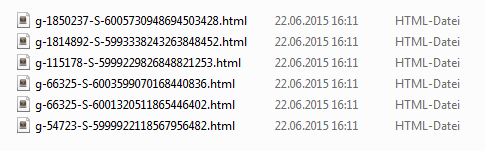
\includegraphics{./images/postdownload.png}
\caption{Heruntergeladne HTML-Seiten der Beiträge der Suchanfragen}
\end{figure}


Es wurden erfolgreich die 6 Dokumente des Forums heruntergeladen, die das Forum auf die 10 Suchanfragen ausgeliefert hat.
Damit ist gezeigt, das es möglich ist, sich automatisch in Foren zu registrieren, einzuloggen und nach bestimmten (firmenspezifischen) Schlagworten für Produkte zu suchen.
\newpage


	\section{Evaluation}
\subsection{Bestimmung der Forenrelevanz}

Es geht darum zu evaluieren, ob eine Vorhersage darüber getroffen werden kann, wie groß eine Forendatenbank und wie relevant dieses Forum für ein jeweiliges Unternehmen ist.

Es wird zunächst die Datenbankgröße bestimmt wie in Kapitel [] beschrieben. Die Testdatenbank wurde in 3 Segemente geteilt. Segement 1 enthält nur Beiträge aus Forum 1, Segement 2 nur aus Forum 2 und Segement 3 nur Beiträge aus Forum 3. 
Segement 1 und 2 beinhalten englische Beiträge, wohingegen Segement 3 meist deutsche Beiträge enthält. Die Postanzahl aller 3 Segemente ist bekannt. Um eine realistische Einschätzung zu erhalten, wie zuverlässig die Vorhersage der Gesamtdatenbankgröße ist, wurde der Test für jedes Segement 3 mal wiederholt. Ein Testdurchlauf besteht aus 3 mal 500 zufälligen Wörtern, die an die Datenbank in der passenden Sprache gesendet werden. Die ermittelten Datenbankgrößen nach 500 Wörtern werden addiert, durch die Gesamtanzahl der Testläufe dividiert und danach mit der bekannten Gesamtanzahl der Posts in dem Datenbanksegment verglichen.

\begin{table}[h!]
\begin{tabular}{ | p{3cm} | p{3cm} | p{3cm}| p{3cm} |} \hline
Durchlauf & Anzahl Dok in S1 & Anzahl Dok in S2 & Anzahl Dok in S3 \\ \hline
1 & 12572 & 18374 & 8079 \\ \hline
2 & 10400 & 21155 & 7896 \\ \hline
3 & 15017 & 20952 & 8343 \\ \hline
Arith. Mittel & 12663 & 20160 & 8016 \\ \hline
org. Größe & 12133 & 21221 & 8184 \\ \hline
Fehler & +4\% & -5\% & -1\% \\ \hline
\end{tabular}
\caption{Ermittelung der Datenbankgrößen mit zufälligen Wörtern}
\end{table}

Der Fehler beträgt maximal 5\% . Dieses bestätigten die zwei weiteren Testdurchläufe. Damit ist eine Voraussage einer Forendatenbank bis auf 10\% Differenz genau möglich.

Im nächsten Schritt sollen die einzelnen Produkte im Forum gesucht werden. Dazu werden, wie in Kapitel[] beschrieben, beschreibende Wörter für jedes einzelne Produkt generiert. Diese Keywords werden gesucht und die Datenbankgröße aufgrund des Verhältnisses zwischen überlappenden und einzigartigen Dokumenten, wie in Kapitel[] beschrieben, berechnet. Die zu Testzwecken verwendete Datenbank enthält 21220 Beiträge.

\begin{table}[h!]
\centering 
\begin{tabular}{ | p{3cm} | l |}
\hline
Produkt & Anzahl der Dokumente in DB \\ \hline
CRM & 2386 \\ \hline
HCM & 3138 \\ \hline
ECOM & 3641 \\ \hline
LVM & 1769 \\ \hline
Gesamt & 10934 \\ \hline
\end{tabular}
\caption{Anzahl der Dokumente je Kategorie in der Testdatenbank. Der Rest der Beiträge konnte keinem Produkt eindeutig zugeordnet werden.}
\end{table}

\newpage

\begin{table}[h!]
\begin{tabular}{ | p{3cm} | l | l |}
\hline
Produkt & Berechnete Anzahl der Dokumente in DB & Fehler\\ \hline
CRM & 3800 & +59 \%\\ \hline
HCM & 9668 & +338 \% \\ \hline
ECOM & 10604 & +265 \%\\ \hline
LVM & 39541 & +2235 \%\\ \hline
\end{tabular}
\caption{Errechnete Datenbankgröße nach Produkt mit Suchworten nach tf-idf Maß}
\end{table}

Zu verzeichnen ist, dass vom Programm die Größe der einzelnen Produktkategorien maßlos überschätzt wurde. Deshalb wird zur Ergebnisverbesserung ein zusätzlicher Schritt eingefügt. Es werden wie bisher die Keywords zu den jeweiligen Produkten im Forum gesucht, jedoch bevor der Post zur Berechnung des Gesamtkorpus beiträgt, durch einen Klassifizierungsservice \cite{n2o} analysiert. Dieser bestimmt aus einem gegebenen Text auf Grundlage der selben Broschüren die zur Berechnung der tf-idf- Keywords verwendet werden, welchem Produkt der Beiträge am ehesten entspricht.

\begin{figure}[h!]
\begin{lstlisting}[language=HTML5]
http://192.168.42.54:9001/predictions?text=Hi, I want to by an CRM product
\end{lstlisting}
\caption{Senden eines Testtextes an den Analyseservice}
\end{figure}

\newpage

\begin{figure}[h!]
\begin{lstlisting}[language=HTML5]
{
"product": [
{
"product": "CRM",
"prob": 0.9999979024787202
},
{
"product": "ECOM",
"prob": 0.0000020975212798552666
},
{
"product": "LVM",
"prob": 3.0982005787342066e-25
},
{
"product": "None",
"prob": 2.2462124385020632e-66
},
{
"product": "HCM",
"prob": 1.5018464896178129e-218
}
]
}
\end{lstlisting}
\caption{Antwort des Analyseservices mit entsprechender Klassifizierung des Textes}
\end{figure}

Der Beitragstext (Abbildung 18) würde als CRM Beitrag richtig eingestuft werden. Wenn gerade die CRM Forendatenbankgröße berechnet werden sollte, wird dieser Beitrag mit in die Berechnung einfließen. Alle Beiträge die als nicht CRM Beiträge eingestuft werden, werden in dieser spezifischen Ermittlung nicht betrachtet.\\
Mit maximal 100 generierten Keywords, gewichtet nach der höchsten tf-Idf, werden folgende Resultate erreicht:

\begin{table}[h!]
\begin{tabular}{ | p{3cm} | l | l |}
\hline
Produkt & Berechnete Anzahl der Dokumente in DB & Fehler \\ \hline
CRM & 2270 & -5\% \\ \hline
HCM & 2730 & -14 \% \\ \hline
ECOM & 4388 & +17\% \\ \hline
LVM & 1670 & -5\% \\ \hline
\end{tabular}
\caption{Errechnete Datenbankgröße je Produkt mit sortierten tf-idf Wörtern und Analyseservice}
\end{table}

Die anderen 2 Testsegmente der Datenbank konnten mit ähnlich genauen Fehlern überprüft werden.
Ein Fehler von maximal 20\% mit nur maximal 100 Suchanfragen ist eine zufriedenstellende Größe. Aus der Datenbankgröße und den spezifischen Produktdatenbankgrößen lässt sich bestimmen, ob das Forum zum Verkauf eines Produktes geeignet ist oder nicht.

	%\section{Schlussfolgerung}

%Der Anteil der gesamten klassifizierbaren Beiträge zur Gesamtdatenbankgröße sollte mindestens 30 \% betragen, damit schnell verkaufsträchtige Posts gefunden werden. Hingegen, sollte der Anteil von spezifischen Posts zur Gesamtdatenbankgröße nicht unter 10 \% fallen, da sonst der Aufwand und die Zeit, diese Beiträge der Kategorie zu erfassen, nicht im Verhältnis zum Gewinn stehen. So wäre in diesem Fall der Teil der Datenbank für CRM , ECOM und HCM Beiträgen geeignet.\\
%Im Bezug auf die Registrierung in jedem Forum könnte es, gerade bei neueren Foren Probleme geben. In manchen Fällen werden Registrierungsanfragen noch mit zusätzlichen Sicherheitsmechanismen wie reCaptcha geschützt. Diese sind in der bisherigen Implementierung noch nicht umgangen worden, was ein Registrieren bei diesen Webseiten unmöglich macht. Wird eine Registrierung in diesen Foren gewünscht, kann die Arbeit von Google herangezogen werden, in dem sie ihre eigenen reCaptcha automatisch von Programmen lösen lassen. Das richtig gelöste reCaptcha zusammen mit den anderen gültigen Registrierungsparametern erlaubt dann ein automatisches Registrieren in solchen Foren. Sollte der Registrierungsvorgang dennoch nicht funktionieren, können händisch ein Nutzeraccount angelegt, verifiziert und diese Daten für einen Login benutzt werden.\\
%Es ist wie gezeigt möglich, sich in Internetforen anzumelden und zu registrieren, sowie Beiträge passend zu Firmenprodukten aus dem Forum zu extrahieren.
%Auch ist es möglich,wenn auch mit kleinem Fehler, die Datenbankgröße des Forums durch Suchanfragen zu bestimmen sowie eine Aussage über die Relevanz eines Forums für ein Unternehmen zu generieren. Dieser Ansatz ermöglicht, das Problem der Datenknappheit für das Noise to Opportunity Produkt zu lösen, sowie rein theoretisch programmatisch Webseiten des Private Webs zu indizieren, was vorher nicht möglich war. Ein Problem besteht darin, dass die bereitgestellten Email-Adressen von der Internetseite 10minutemail \footnote{https://10minutemail.net/ checked: 10.06.2015} nicht zum Registrieren im Forum benutzt werden können. Das kann passieren, wenn zu viele Spam-Accounts mit Emails von diesem Anbieter im Forum erstellt wurden. Um das Problem zu lösen, muss entweder ein Account manuell erstellt, oder das Programm so verändert werden, dass es sich mit einem anderen Email-Provider registriert. Jedoch muss das Programm auch bei diesem neuen Provider die Möglichkeit haben, die Links in der Aktivierungsmail zu bestätigen.
%Sollte bei dem Login oder Registrierungsprozess von der Webseite noch zusätzliche Parameter per Javascript eingefügt werden, wird dieses vom Programm noch nicht registriert.
%Zu beachten und respektieren sind die geltenden AGB's der Internetforen, die untersucht werden sollen. Ist ein programmtechnisches Durchsuchen dieser Webseite untersagt, sollte dieses Programm nicht eingesetzt werden.

\section{Schlussfolgerung}
Unter den 100 getesteten Internetforen konnte ein erfolgreicher Registrierungsprozess bei 76\% der nachgebauten Registrierungsseiten der Foren festgestellt werden. Bei 82\% der Webseiten konnte sich erfolgreich eingeloggt werden. Dafür wurde manuell bei 6 Webseiten ein Nutzerkonto angelegt und validiert, sich dann aber automatisch mit den generierten Nutzerdaten eingeloggt. Bei 80 \% der Webseiten konnten die Suchform identifiziert und eine Suchanfrage korrekt abgesendet werden. Damit sollte es bei mindestens 63 \% (76 * 0.82) der Foren die im Internet verfügbar sind, möglich sein, diese programmtechnisch zu durchsuchen.
Um eine Aussage darüber treffen zu können, wie relevant dieses Forum im Endeffekt für das Verkaufen eines Firmenproduktes ist, wird neben der Klassifizierung des Produktes eines Beitrags der in diesem Beitrag ausgedrückte Kaufwunsch gespeichert. Dieser Kaufwunsch ist ein nummerischer Wert, den der Klassifizierungsservice von Berger und Hennig\cite{n2o} bei jeder Produktbestimmung eines Beitrages mit ausliefert. Für jeden extrahierten Beitrag, der einem Unternehmensprodukt zugeordnet werden kann, wird dieser Wert addiert und zum Schluss durch die Anzahl der gefundenen Produktbeiträge dividiert. Dabei ergibt sich folgende Verteilung: 

\begin{table}[h!]
\centering
\begin{tabular}{ | p{3cm} | l |}
\hline
\textbf{Produkt} & \textbf{Kaufwunsch}\\ \hline
CRM & 79\% \\ \hline
HCM & 52\% \\ \hline
ECOM & 54\% \\ \hline
LVM & 57\% \\ \hline
\end{tabular}
\caption{Errechneter Kaufbedarf für jede Produktkategorie}
\end{table}

Das bedeutet, dass fast 80\% der CRM Beiträge in der Testdatenbank mit 22120 Beiträgen, einen Kaufbedarf äußern. Demnach drücken in der getesteten Datenbank 1816 Beiträge einen starken Kaufbedarf an einem CRM-Produkt aus. Dem Verkäufer wird eine Statistik generiert und angezeigt. Er kann dann entscheiden, ob dieses Forum für den Vertrieb seines Produktes geeignet scheint. Das Verhältnis von produktspezifischen Beiträgen zu Gesamtdatenbankgröße sollte nicht unter 5\% fallen, da sich dann dieses Forum mit anderen Themen als dem gesuchten Unternehmensprodukt befasst. Weiterhin sollte bei mindestens 30\% der klassifizierten Beiträge ein Kaufbedarf erkennbar sein, da sonst zwar produktspezifische Beiträge gefunden werden können, diese dem Verkäufer jedoch nichts bringen, da er den Autoren kein Produkt verkaufen kann. Diese Zahlen müssten mit realen Verkäufen in realen Internetforen evaluiert werden, stellen aber eine gute Richtlinie für eine Forenrelevanz dar.

\section{Ausblick}
Im Bezug auf die Registrierung in Foren könnte es, gerade bei neueren Foren, Probleme geben. In manchen Fällen werden Registrierungsanfragen noch mit zusätzlichen Sicherheitsmechanismen wie `reCaptcha` geschützt. Diese sind in der bisherigen Implementierung noch nicht umgangen worden, was ein Registrieren bei diesen Foren unmöglich macht. Wird eine Registrierung in diesen Foren gewünscht, kann die Arbeit von Google herangezogen werden, in der sie ihre eigenen `reCaptcha` automatisch von Programmen lösen lassen\cite{goodfellow2013multi}. Das richtig gelöste `reCaptcha`, zusammen mit den anderen gültigen Registrierungsparametern, erlaubt dann ein automatisches Registrieren in solchen Foren. Sollte der Registrierungsvorgang dennoch nicht funktionieren, kann händisch ein Nutzeraccount angelegt, verifiziert und können diese Daten für einen Login benutzt werden.\\
Ein Problem besteht, wenn die bereit gestellten Email-Adressen von der Internetseite 10minutemail \footnote{https://10minutemail.net/ checked: 10.06.2015} in manchen Foren nicht zum Registrieren benutzt werden können. Das kann passieren, wenn zu viele Spam-Accounts mit Emails dieses Anbietes im Forum erstellt wurden. Um das Problem zu lösen, muss entweder ein Account manuell erstellt oder das Programm so verändert werden, dass es sich mit einem anderen Email-Provider registriert. Jedoch muss das Programm auch bei diesem neuen Provider die Möglichkeit haben, die Links in der Aktivierungsmail zu bestätigen.
Sollten beim Login- oder beim Registrierungsprozess von der Webseite noch zusätzliche Parameter per Javascript eingefügt werden, wird dieses vom Programm noch nicht registriert.\\
In einer Testphase sollten Datenbankgrößen ausgerechnet werden, um abzuschätzen, ob die Formel zur Berechnung der Datenbankgröße die Größen richtig berechnet. Sollte dies nicht der Fall sein, können eine andere Formel und zusätzlich eine Gewichtung der Suchwörter nach dem Zipf'schen Gesetz \cite{leopold2002zipfsche} der jeweiligen Sprache implementiert und getestet werden\cite{jiang2009selectivity}.
Zu beachten und zu respektieren sind die geltenden AGBs der untersuchten Internetforen. \textbf{Ist ein programmtechnisches Durchsuchen dieser Webseite untersagt, sollte dieses Programm nicht eingesetzt werden!}

	
	\section{Hintergrund}

Im Rahmen des Bachelorprojektes am Hasso-Plattner-Institut wurde innerhalb eines Jahres die Softwarelösung `Noise to Opportunity` in einer Gruppe von 8 Personen entwickelt. `Noise to Opportunity` durchsucht soziale Medien und analysiert die gefundenen Beiträge. Drücken diese einen Kaufwunsch aus und können einem Unternehmensprodukt zugeordnet werden, werden diese an Vertreter weitergeleitet, die auf den Verkauf dieses Produktes spezilaisiert sind. Ich habe mich mit der Datenakquise beschäftigt. Dazu habe ich eine Vielzahl von Webseiten analysiert um die Registrierungs-, Einlogg- und Suchprozesse zu verstehen und programmtechnisch nachzubauen. Bei dieser Tätigkeit ist aufgefallen, dass die meisten Internetforen eine ähnliche Struktur besitzen. Anfänglich war die Herausforderung, sich mit einem händisch angelegten Nutzeraccount im Forum automatisch anzumelden und das Forum zu durchsuchen. Die Analyse der Webseiten ließ sich wiederholende Prozesse erkennen, so entstand die Idee, sich auch automatisch registrieren zu wollen.
Viele der Registrierungsformen besitzen gleiche Attributnamen, die sie in dem HTML-Quellcode identifizieren. Der Registrierungsprozess folgt dem gleichen Schema und lässt sich demnach genau wie das Einloggen und das Suchen automatisieren. Es entstand die Idee ein Programm zu entwickeln, das automatisch Internetinhalte hinter POST- und GET- Formularen und des Deep- und Private Webs indizieren könnte. Wir sahen die Möglichkeit, eine Voraussage darüber zu treffen, wie viele Beiträge und wie viele Beiträge zu einem bestimmten Produkt in einem Forum vorhanden sind.
Daraus entwickelte sich die These dieser Arbeit, ob es möglich sei, abzuschätzen wie verkaufsrelevant das Forum für Unternehmensprodukte ist.

\subsection{Related Work}

Jianuguo Lu \cite{lu2008efficient} entwickelt in seiner Arbeit eine Formel, die eine Bestimmung der Datenbankgröße ermöglicht, wenn die Datenbank nur über ein Suchanfragen Interface angefragt werden kann. Er beschreibt die Abhängigkeit von der Anzahl der Suchanfragen zur Anzahl der Einträge, die auf eine Suchanfrage zurückgegeben werden. Getestet wird an Datenbanken mit bekannten Größen. Dabei wird eine Konvergenz zur realen Datenbankgröße ab 200 Suchanfragen festgestellt. Die Formel aus dem heterogenen Modell (Seite 1) ist die Grundlage für die Errechnung der Forendatenbank-Größe, sowie für die Errechnung der Datenbank-Größe für ein spezifisches Firmenprodukt.

Patrick Hennig und Philipp Berger \cite{n2o} untersuchen in ihrer Arbeit die Möglichkeit aus Social-Media-Beiträgen, diejenigen herauszufiltern, die einen Kaufbedarf ausdrücken und diese gleichzeitig einem Produkt zuzuordnen. Dabei untersuchen sie die Richtigkeit verschiedener Algorithmen zum Erkennen des Kaufbedarfs (Seite 12) sowie Algorithmen zum Klassifizieren des Produktes (Seite 13). Dieser implementierte Service liefert in dieser Arbeit den Ausgangspunkt für die Ermittelung der Datenbankgröße für ein Firmenprodukt.

Juan Ramos \cite{ramos2003using} beschreibt in seiner Arbeit die Relevanz des `tf-idf-Algorithmus` zur Gewinnung von Schlagworten aus Dokumenten. Er zeigt, dass die alleinige Gewichtung der Wörter nach Anzahl der Wortvorkommen keine relevanten Schlagworte generiert, sondern erst die Gewichtung von Wortvorkommen im Verhältnis zum Vorkommen in den Dokumenten. Dieser Ansatz der tf-idf Wortgenerierung wird eingesetzt, um passende Produktschlagworte aus den Unternehmensunterlagen zu gewinnen. Die Studie belegt, dass diese Worte ein Produkt gut klassifizieren, was an den Evaluationsergebnissen bestätigt werden kann.

Ian J. Goodfellow, Yaroslav Bulatov, Julian Ibarz, Sacha Arnoud, Vinay Shet \cite{goodfellow2013multi} erläutern in ihrer Arbeit, wie durch den Versuch bei Google-Street-View \footnote{https://www.google.com/maps/views/streetview?gl=de\&hl=de checked: 20.06.2015}, die Hausnummern automatisch zu erkennen, ein Algorithmus entstand, der `reCaptchas` mit Wahrscheinlichkeit von 99,8\% richtig ausfüllt. Bei der Registrierung in Foren wird zum Teil durch diese `reCaptchas` validiert, ob sich ein Mensch versucht anzumelden. Soll dieses automatisiert passieren, kann der Algorithmus aus der Arbeit eine gute Grundlage zur Implementierung bieten.

In der Arbeit von Edda Leopold \cite{leopold2002zipfsche} wird beschrieben, wie das Zipf'sche Gesetz eine Verteilung der Worthäufigkeiten in einer Sprache generieren kann. Dieses könnte in Kombination mit der Errechnung der Gesamtdatenbankgröße ein besseres Ergebnis erzielen, wenn sich bei einer längeren Evaluation herausstellt, dass die Datenbankgrößen falsch abgeschätzt werden. Sollte das der Fall sein, könnten nur mittels häufig vorkommender Wörter der Sprache gesucht werden, oder die Gewichtung für überlappende Dokumente bei Wörtern aus der unteren oder oberen Zipf Verteilung geändert werden. 

Sonali Gupta, Komal Kumar Bhatia \cite{gupta2014comparative}, sowie Jayant Madhavan u.a \cite{madhavan2008google} beschreiben in ihrer Arbeit die Idee, Teile des Deep Webs zu durchsuchen, indem sie valide Suchanfragen aus dem Suchinterface generieren und an die Webseite absenden. Dazu analysieren sie die Suchformen, füllen sie mit Suchworten und diskutieren die Vor- und Nachteile von breiten- zu tiefenorientierten Crawlern. Sie evaluieren mit wie viel Suchaufwand es möglich ist, einen möglichst großen Anteil der Datenbank zu indexieren. Diese Arbeiten gaben den Anlass dazu, eine Metrik dafür zu entwickeln, welche Formen zum Einloggen und Registrieren vorhanden sind, sowie programmtechnisch die Suchform zu erkennen und anhand der Links als DokumentID die Datenbankgröße zu generieren.


	\clearpage
	%%% BIBLIOGRAPHY
	%\bibliographystyle{babunsrt3-fl}
	\nocite{*}
	\addcontentsline{toc}{section}{Bibliography}
    	\bibliographystyle{babunsrt-fl}
   	\bibliography{projektbib}
   	   	\newpage
   	\section{Anhang}
   	
   	\begin{figure}[ht]
   		\centering
		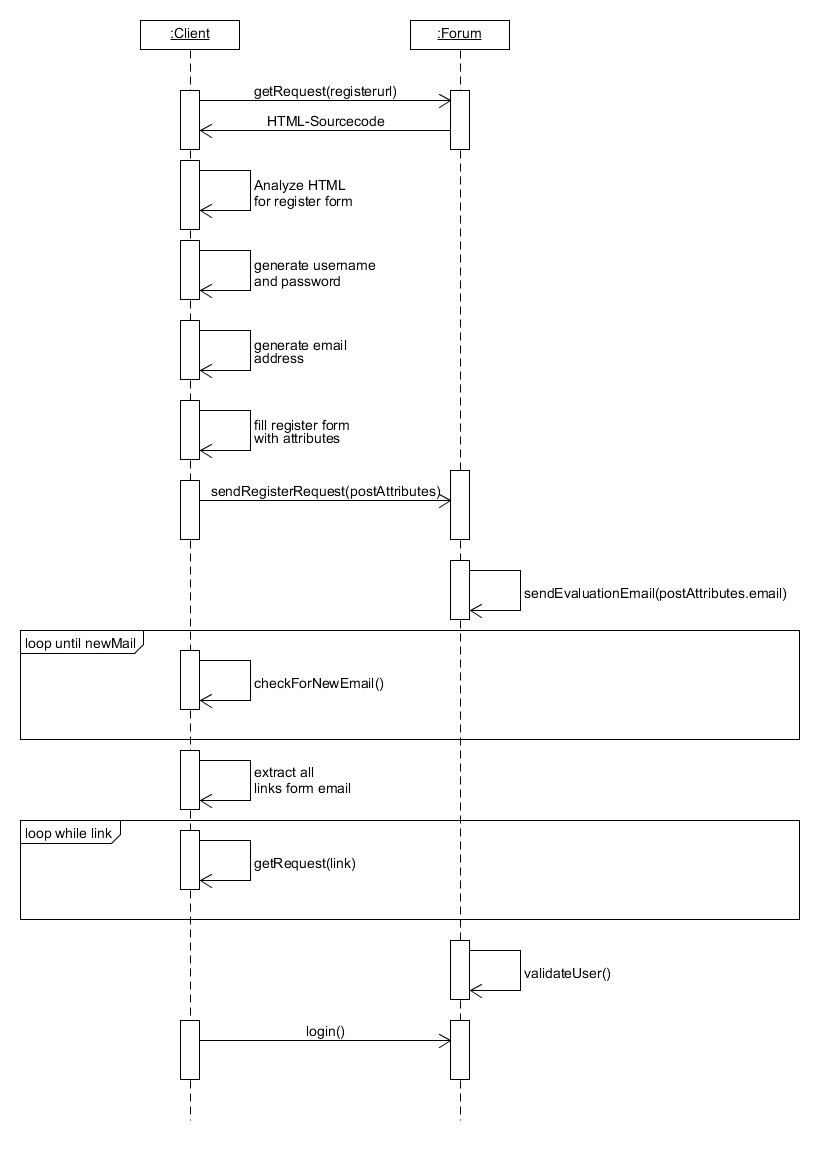
\includegraphics[width=0.76\textwidth,height=\textheight,keepaspectratio]{./diagrams/register_seq.png}
		\caption{Vollständiger Registrierungsablauf}
	\end{figure}
	\newpage
	\begin{figure}[ht]
		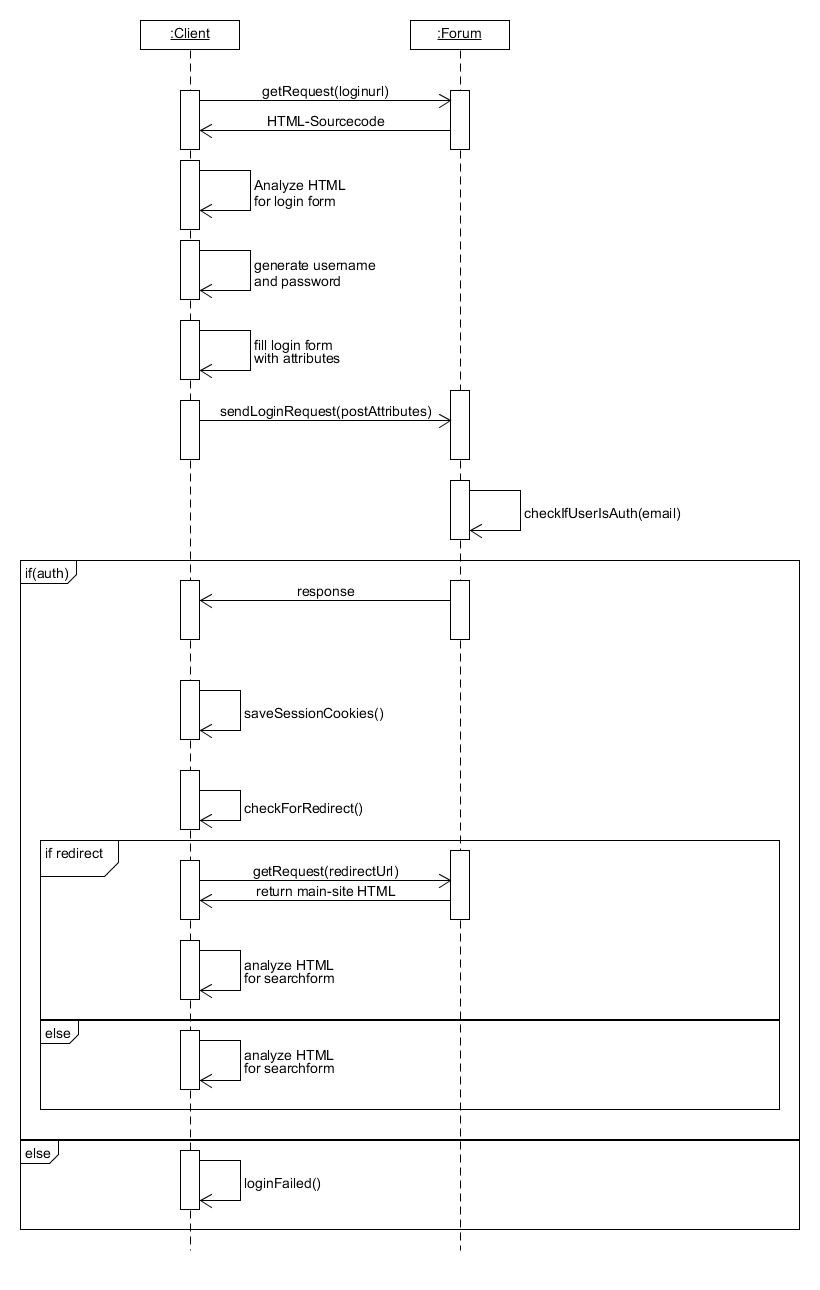
\includegraphics[width=\textwidth,height=\textheight,keepaspectratio]{./diagrams/login_seq.png}
		\caption{Vollständiger Loginablauf}
	\end{figure}
	
	
\end{document}
